\chapter{Results and Analysis}
    \section{Spectrometer Measurement}
    A GUI (graphical user interface) was used to proceed with the experiment. This procedure ensures that the contribution from background noise (room lights and any other ambient sources) were extracted and only the photons emitted by the LED source are considered in the analysis. \\
    
    The experiment was conducted by measuring the spectrum at 0° with the room lights switched on and off to account for dark currents. The dark counts were then subtracted from the signal to filter out ambient photons, including those from room lights and any other external sources.
    
    \begin{figure}[H]
        \centering
        \begin{subfigure}[b]{0.48\textwidth}
            \centering
            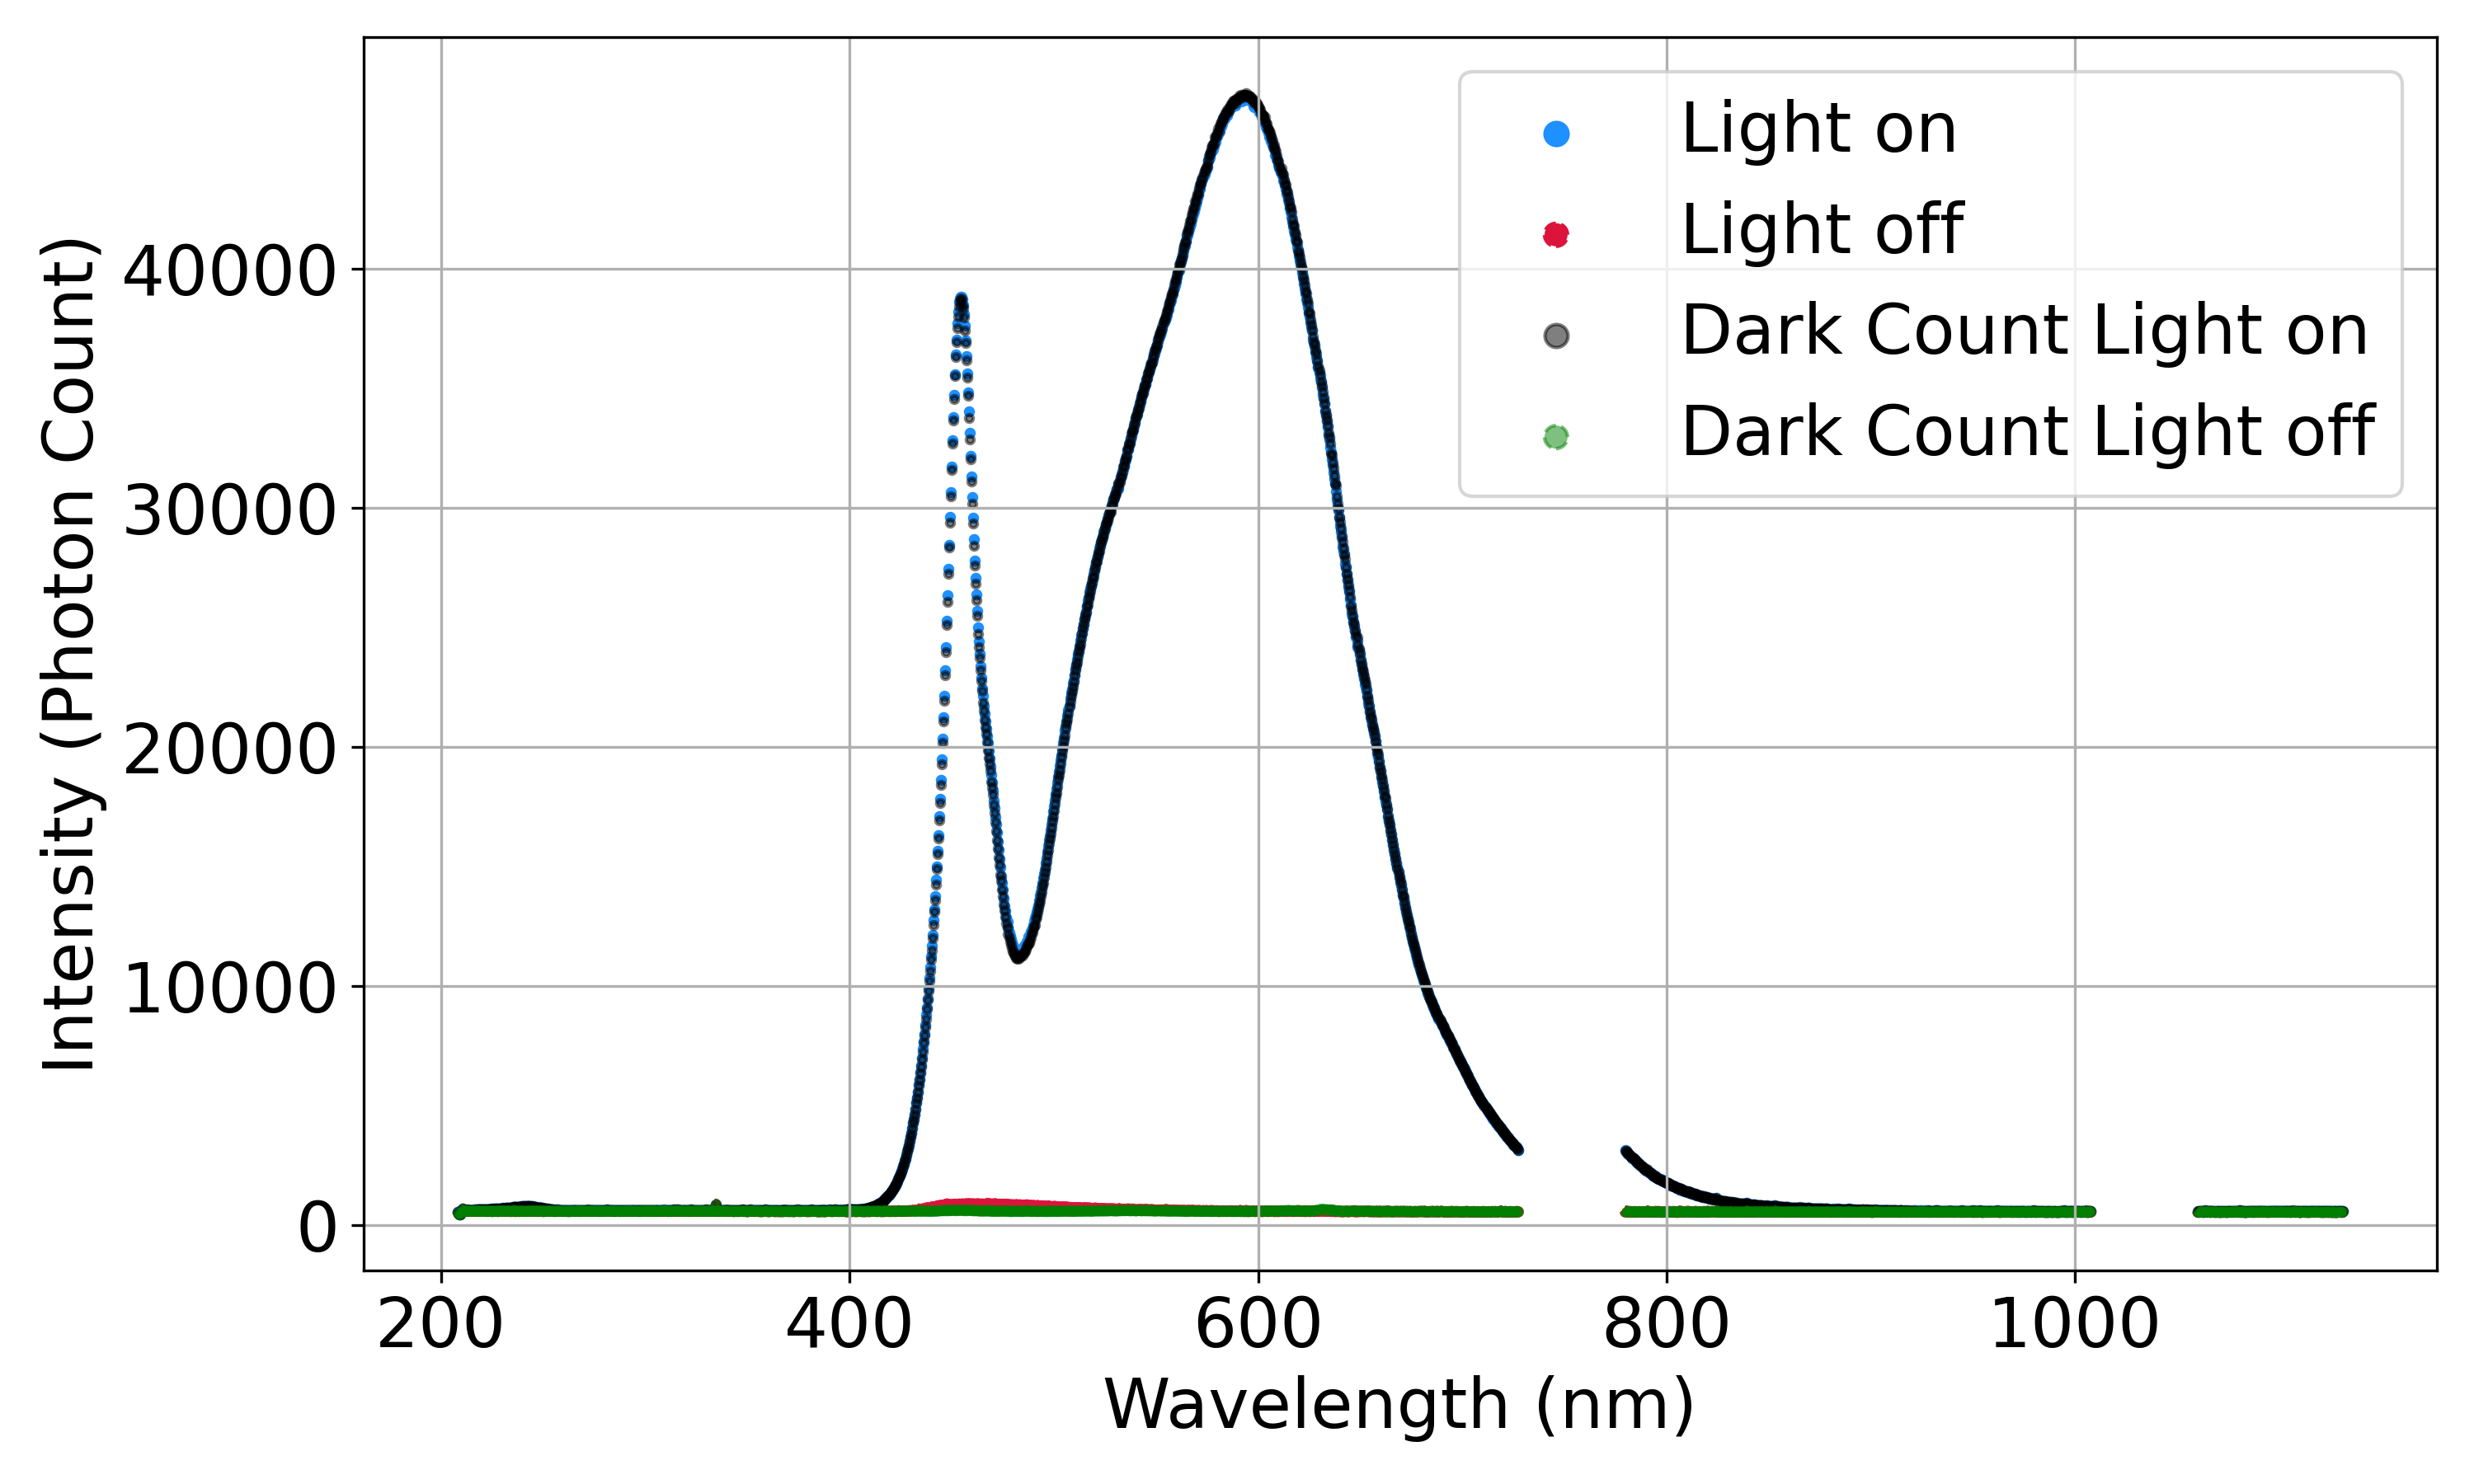
\includegraphics[width=\textwidth, scale=0.35]{Figure/spectrum_high_res.png}
            \caption{Plot of Intensity vs. Wavelength for both lights on and lights off.}
        \end{subfigure}
        \hfill
        \begin{subfigure}[b]{0.48\textwidth}
            \centering
            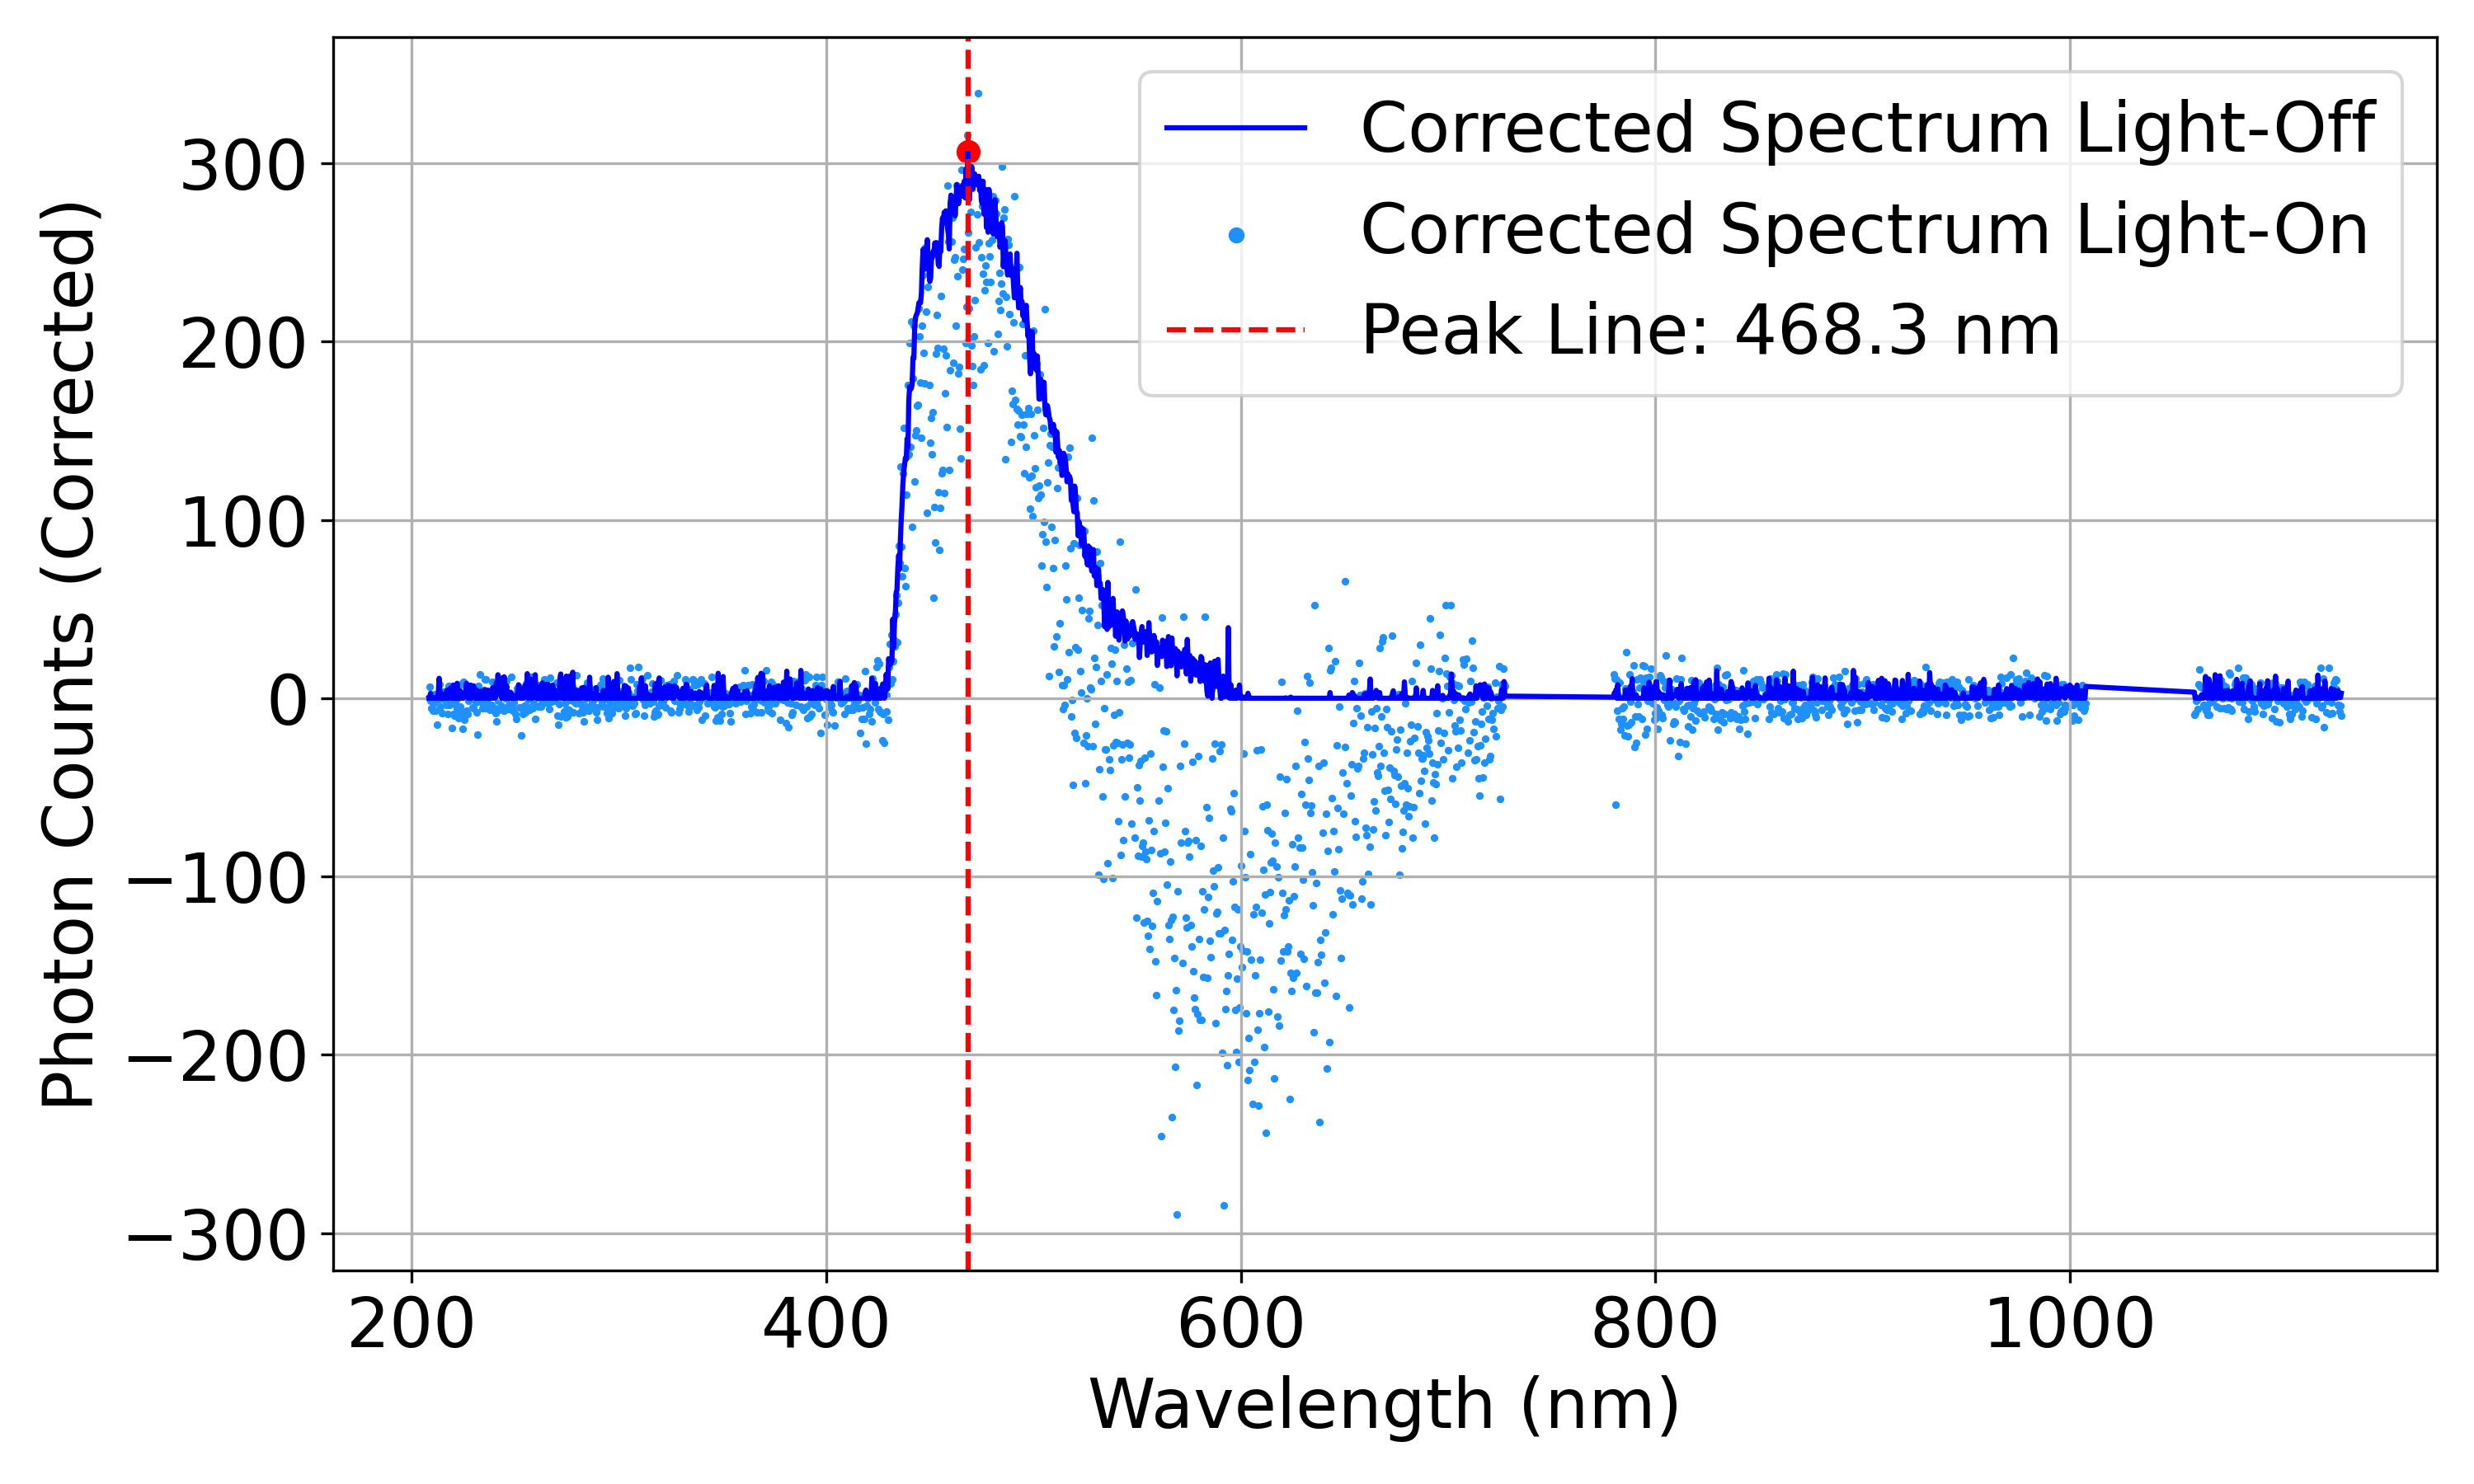
\includegraphics[width=\textwidth, scale=0.35]{Figure/corrected_spectrum_high_res.png}
            \caption{Plot of Corrected Intensity vs. Wavelength showing peak.}
        \end{subfigure}
        \caption{Spectral response comparison.}
        \label{spectral}
    \end{figure}

    The two peaks in the Figure \ref{spectral}(a) occurs because of the spectrum of the room lights which doesn't have anything to do with the experiment. The missing region in both the plots might have happened because the spectrometer has blind spots at those regions. The fluctuations in Figure \ref{spectral}(b) was caused by large amount of photons. 

    

    \section{Radial Symmetry}
    This section aims to verify the radial symmetry of light intensity by recording it at various horizontal and vertical angles while keeping the excitation position fixed. The horizontal angles should cover a range from −18° to 30° with steps of 4° and the vertical angle a range from −6° to 35° with steps of 4°. This has been done with the room lights turned off. \\

    The integrated intensity is plotted in a heatmap where the vertical axis is the horizontal angles and the horizontal axis is the vertical angles. 

    \begin{figure}[H]
        \centering
        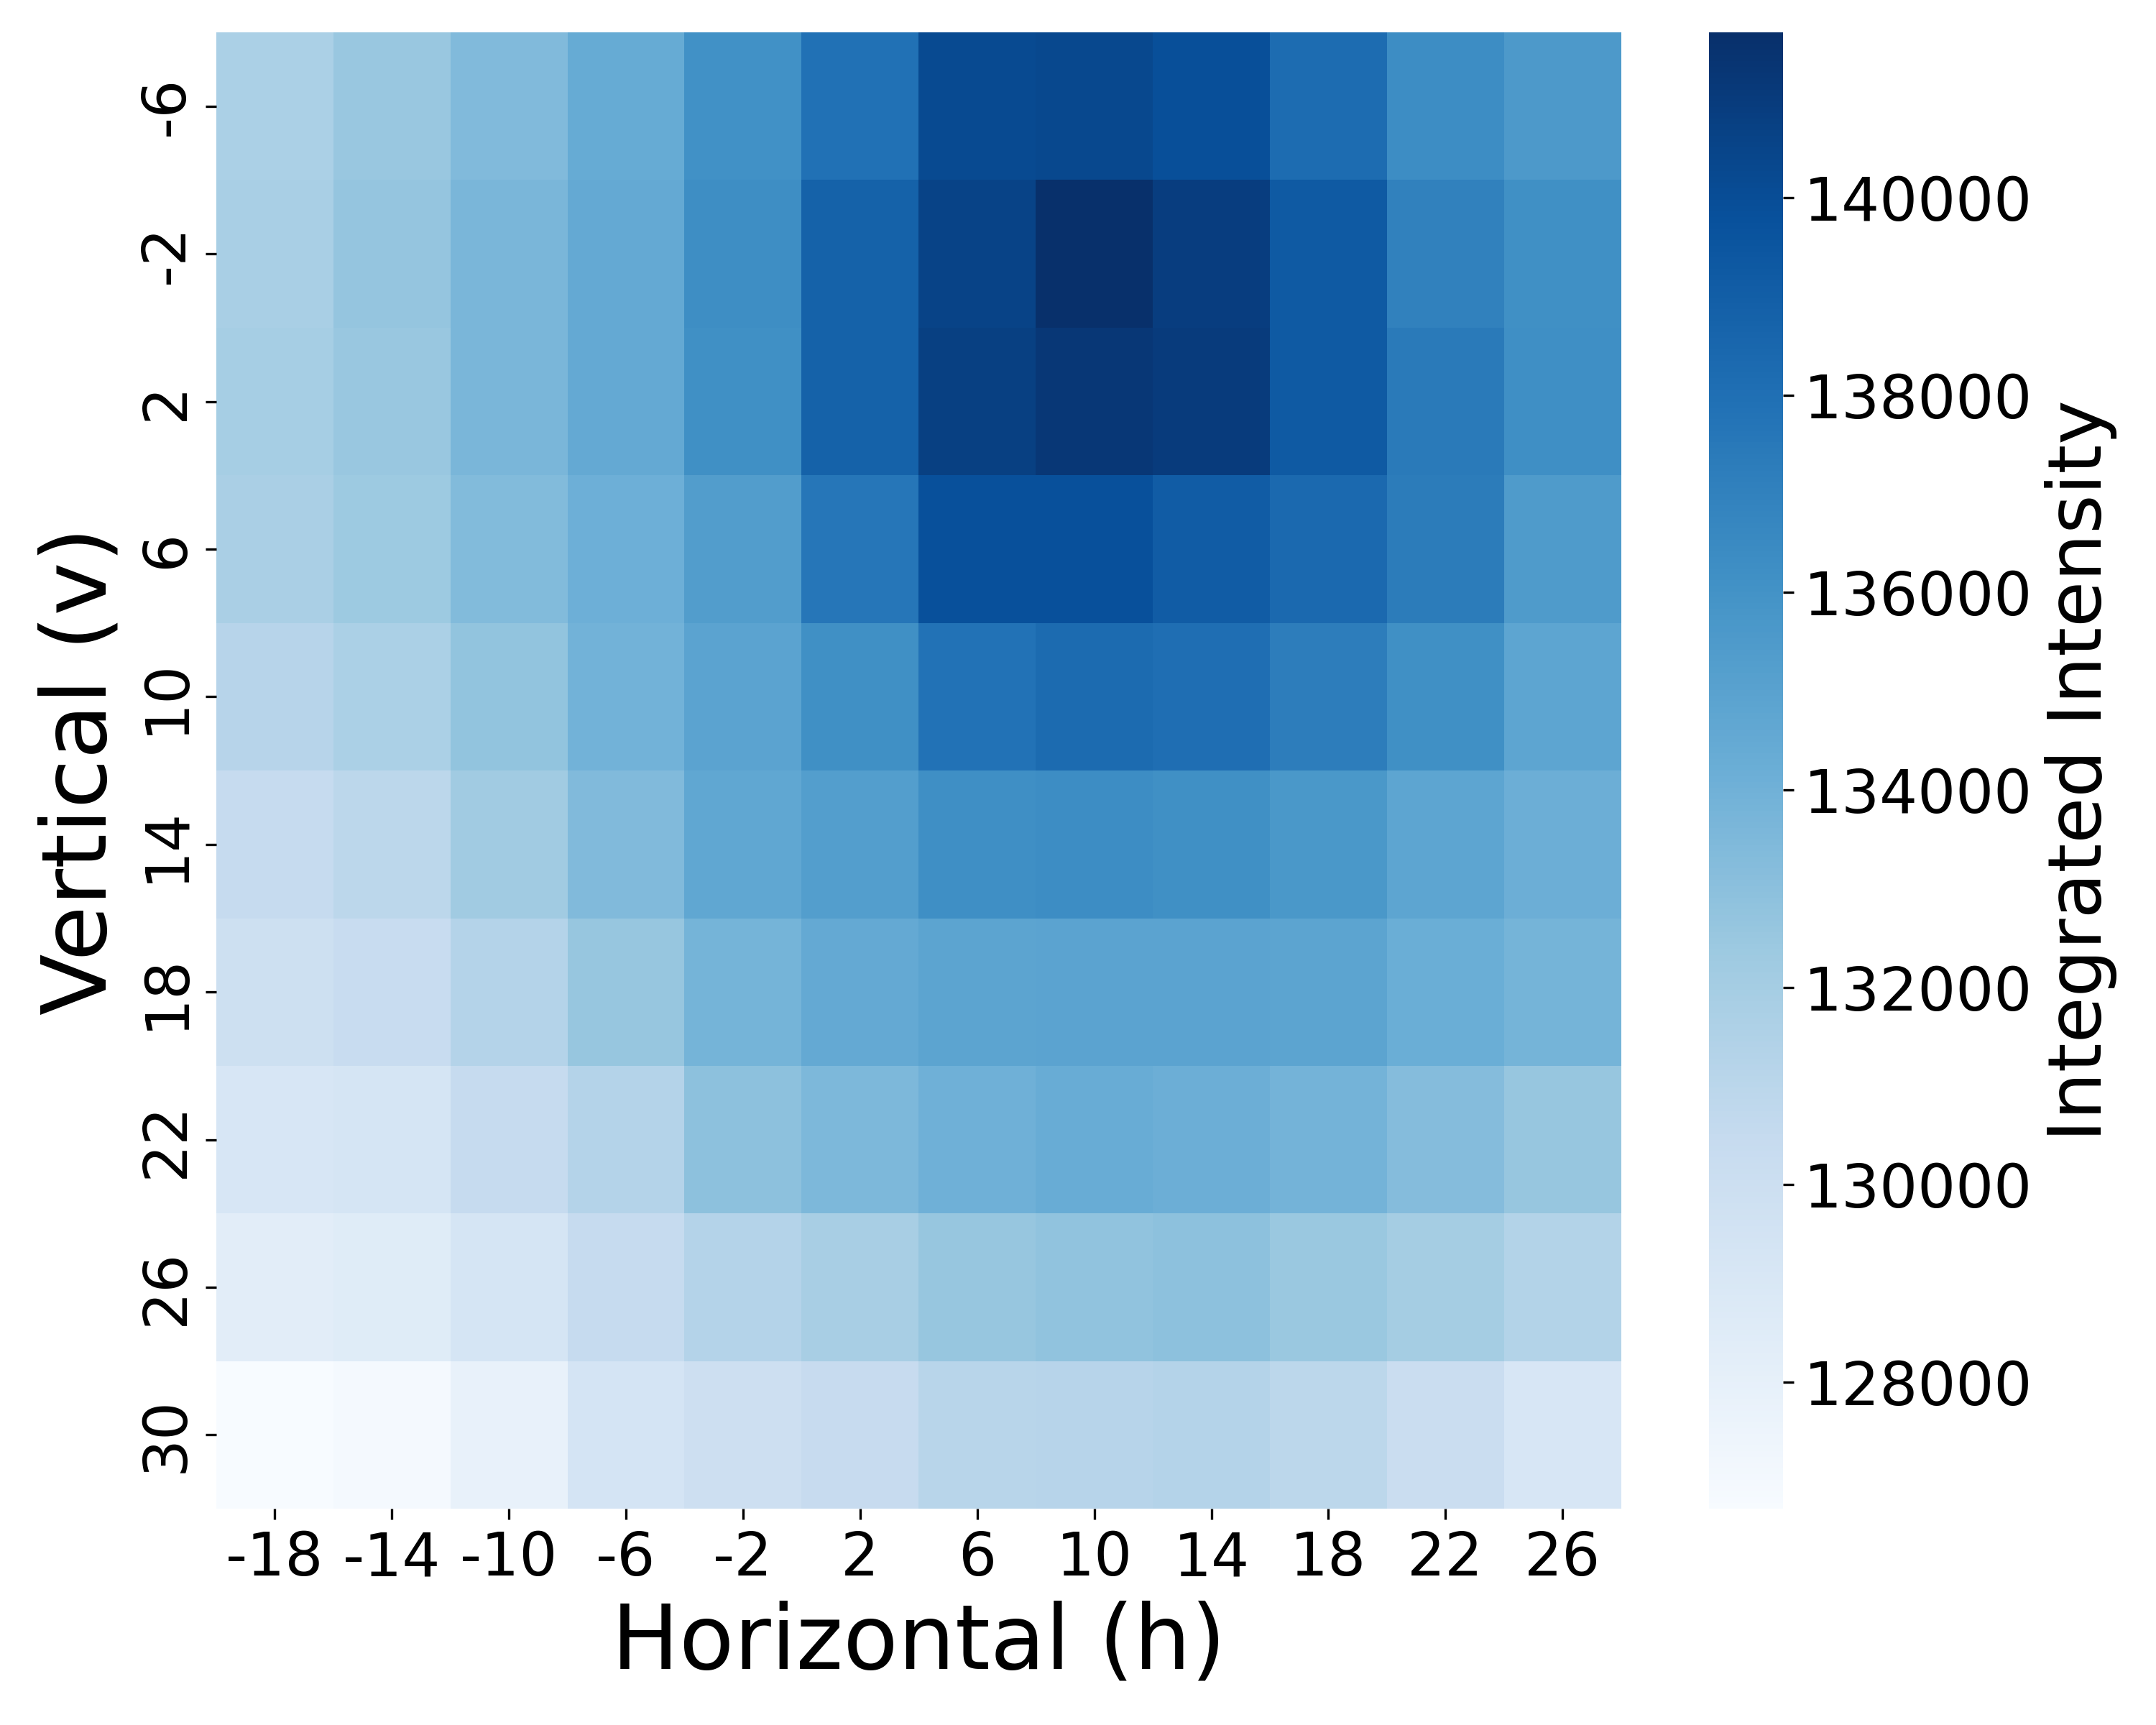
\includegraphics[scale=0.25]{Figure/heatmap.png}
        \caption{Heatmap of the integrated intensity as a function of the horizontal and vertical
        angles.}
        \label{radial}
    \end{figure}

    The heatmap in the Figure \ref{radial} clearly shows that the maximum of the integrated intensity has occurred at horizontal angle from -4° to 0° and vertical angle from 12° to 16° instead of 0°'s. This strongly suggests that the reference frame of the spectrometer is not perfectly centered with respect to the scintillating fiber.
    
    \section{Simulation Analysis}

    In this section, the simulation results from Geant4 are presented which model the behavior of photons traveling through scintillating fibers. The simulation setup involved 50 individual fibers, each excited at 24 different points. These points were spaced 100 mm apart, starting at 2400 mm and ending at 100 mm from the fiber end. This configuration allowed for an analysis of photon behavior at multiple positions along the length of the fiber.\\
    
    The simulation data are divided into core and cladding photons by the position of reflection. To ensure that the simulation data are aligned with physics theory, data with a radial distance from the fiber axis larger than the fiber radius,$r_{min} = 125 mm$ are excluded. The result after selecting the possible data can be seen in Figures \ref{hist_1} (left). \\

    The angle $\theta$ of the emitted photon to the fiber x-axis is an important observable for the analysis, which can be derived from the normalized momentum as follows:
    \[
        \theta = \arccos(p_x)
    \]
    
    Theoretically, the maximum angle $\theta$ can be calculated using Snell's law, where the refractive indices of the fiber materials are as follows: the core $n_{\text{Core}}$ is 1.60, the first cladding $n_{\text{CladdingIn}}$ is 1.49, and the second cladding $n_{\text{CladdingOut}}$ is 1.42.

    \[
    \theta_{\text{MaxCore}} = \arccos\left(\frac{n_{\text{CladdingIn}}}{n_{\text{Core}}}\right) = 21.4^\circ
    \]
    \[\quad \theta_{\text{MaxCladding}} = \arccos\left(\frac{n_{\text{CladdingOut}}}{n_{\text{Core}}}\right) = 27.4^\circ
    \]

    To compare with the data, it can be clearly seen that the theoretical results align with the simulation data in the distribution of $\theta$ for the core and cladding photons shown in Figures \ref{hist_1} (right).
    
    \begin{figure}[H]
        \centering
        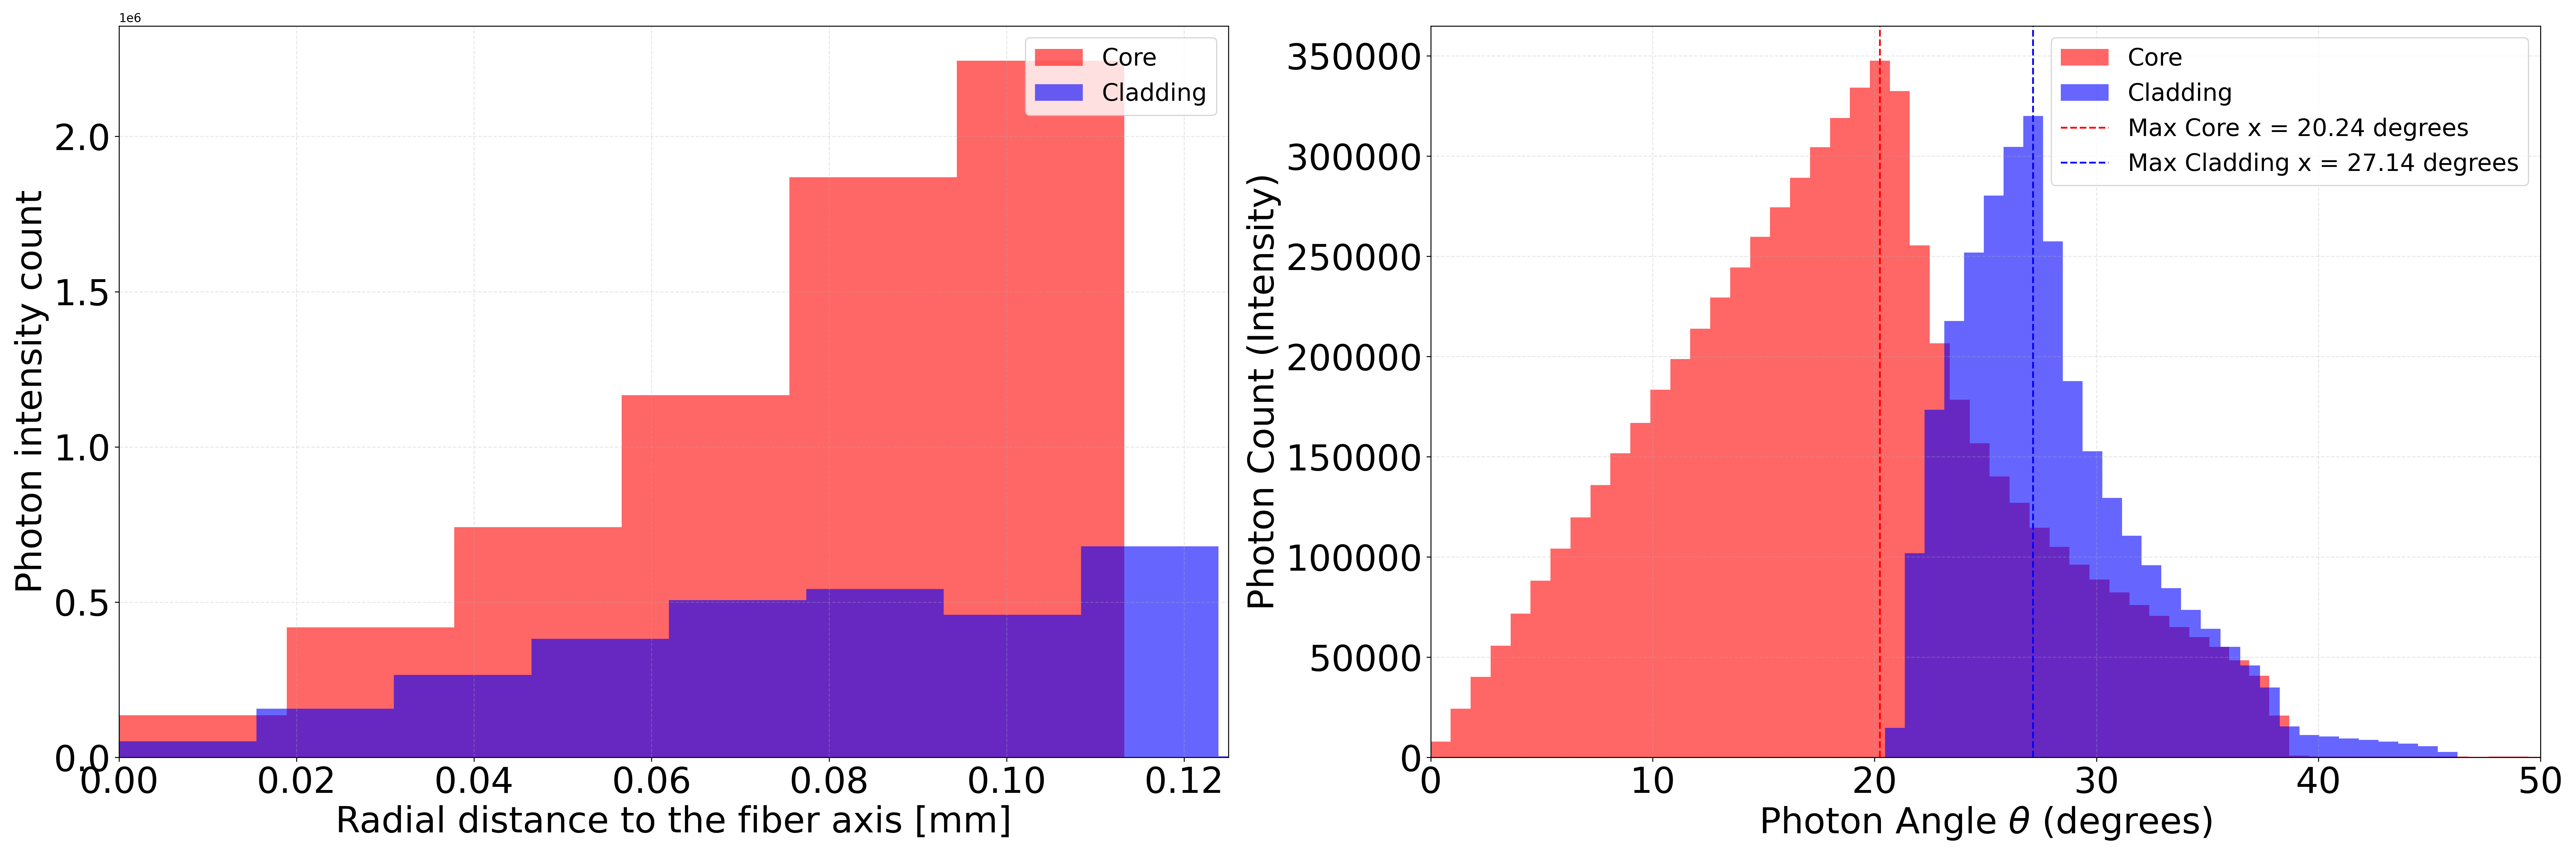
\includegraphics[width=1.0\textwidth]{Figure/photon_combined.png}
        \caption{
        Histogram showing the angular distribution ($\theta$) of photons in the core and cladding from the simulation data. The separation highlights the difference in propagation modes.
        }
        \label{fig:theta_distribution}
    \end{figure}

    From the right histogram, a linear trend is observed from $\theta = 0$ to $\theta_{\text{Max}}$ and then followed by an exponential decrease for values greater than $\theta_{\text{Max}}$. This behavior of the distributions can be explained by the geometry of the incident area and total internal reflection. At smaller angles, photons mostly hit the surface of the fiber. However, as the angle increases, a larger fiber's surface is exposed to the incoming photon.
    After reaching the maximum angle $\theta_{\text{Max}}$, the intensity of photons in the fibers shows an exponential decrease. This drop occurs because photons that are incident at angles greater than $\theta_{\text{Max}}$ happening total internal reflection and thus reducing their contribution to the detected signal. \\ 

%4. �� is to be histogrammed for core and cladding photons (in a plot) and the theoretical maximum angles are to be marked. Where does the supposed linear increase come from? Why are there photons with a higher angle than the maximum angle?

    To further analyze, the minimum distance of the photons to the fiber center should be determined from the simulation data. The minimum distance $r_{\text{min}}$ is obtained through the following formula:

        \[
            r_{\text{min}} = \frac{\abs{{y_{\text{start}} \cdot p_{z_{\text{start}}} - z_{\text{start}} \cdot p_{y_{\text{start}}}}}}{\sqrt{p_{z_{\text{start}}}^2 + p_{y_{\text{start}}}^2}}
        \]
    where \( y \) and \( z \) are the initial positions of the photons, \( p_y \) and \( p_z \) are the initial normalized of their momenta. As shown in Figure \ref{dist_1}, the 2D histogram of the photon counts as a function of \( r_{\text{min}} \) and the photon emission angle \( \theta \) shows a clear gradient. There is an obvious upper bound for the minimum distance \( r_{\text{min}} \) around \( 0.10\,\text{mm} \). Moreover, the upper bound for the emission angle \( \theta \) is around \( 40^\circ \) and \( 48^\circ \) for core and cladding photons, respectively. However, a lower bound in \( r_{\text{min}} \) exists for cladding photons at approximately \( 20^\circ \). \\
    
    \begin{figure}[H]
        \centering
        \begin{subfigure}[b]{0.48\textwidth}
            \centering
            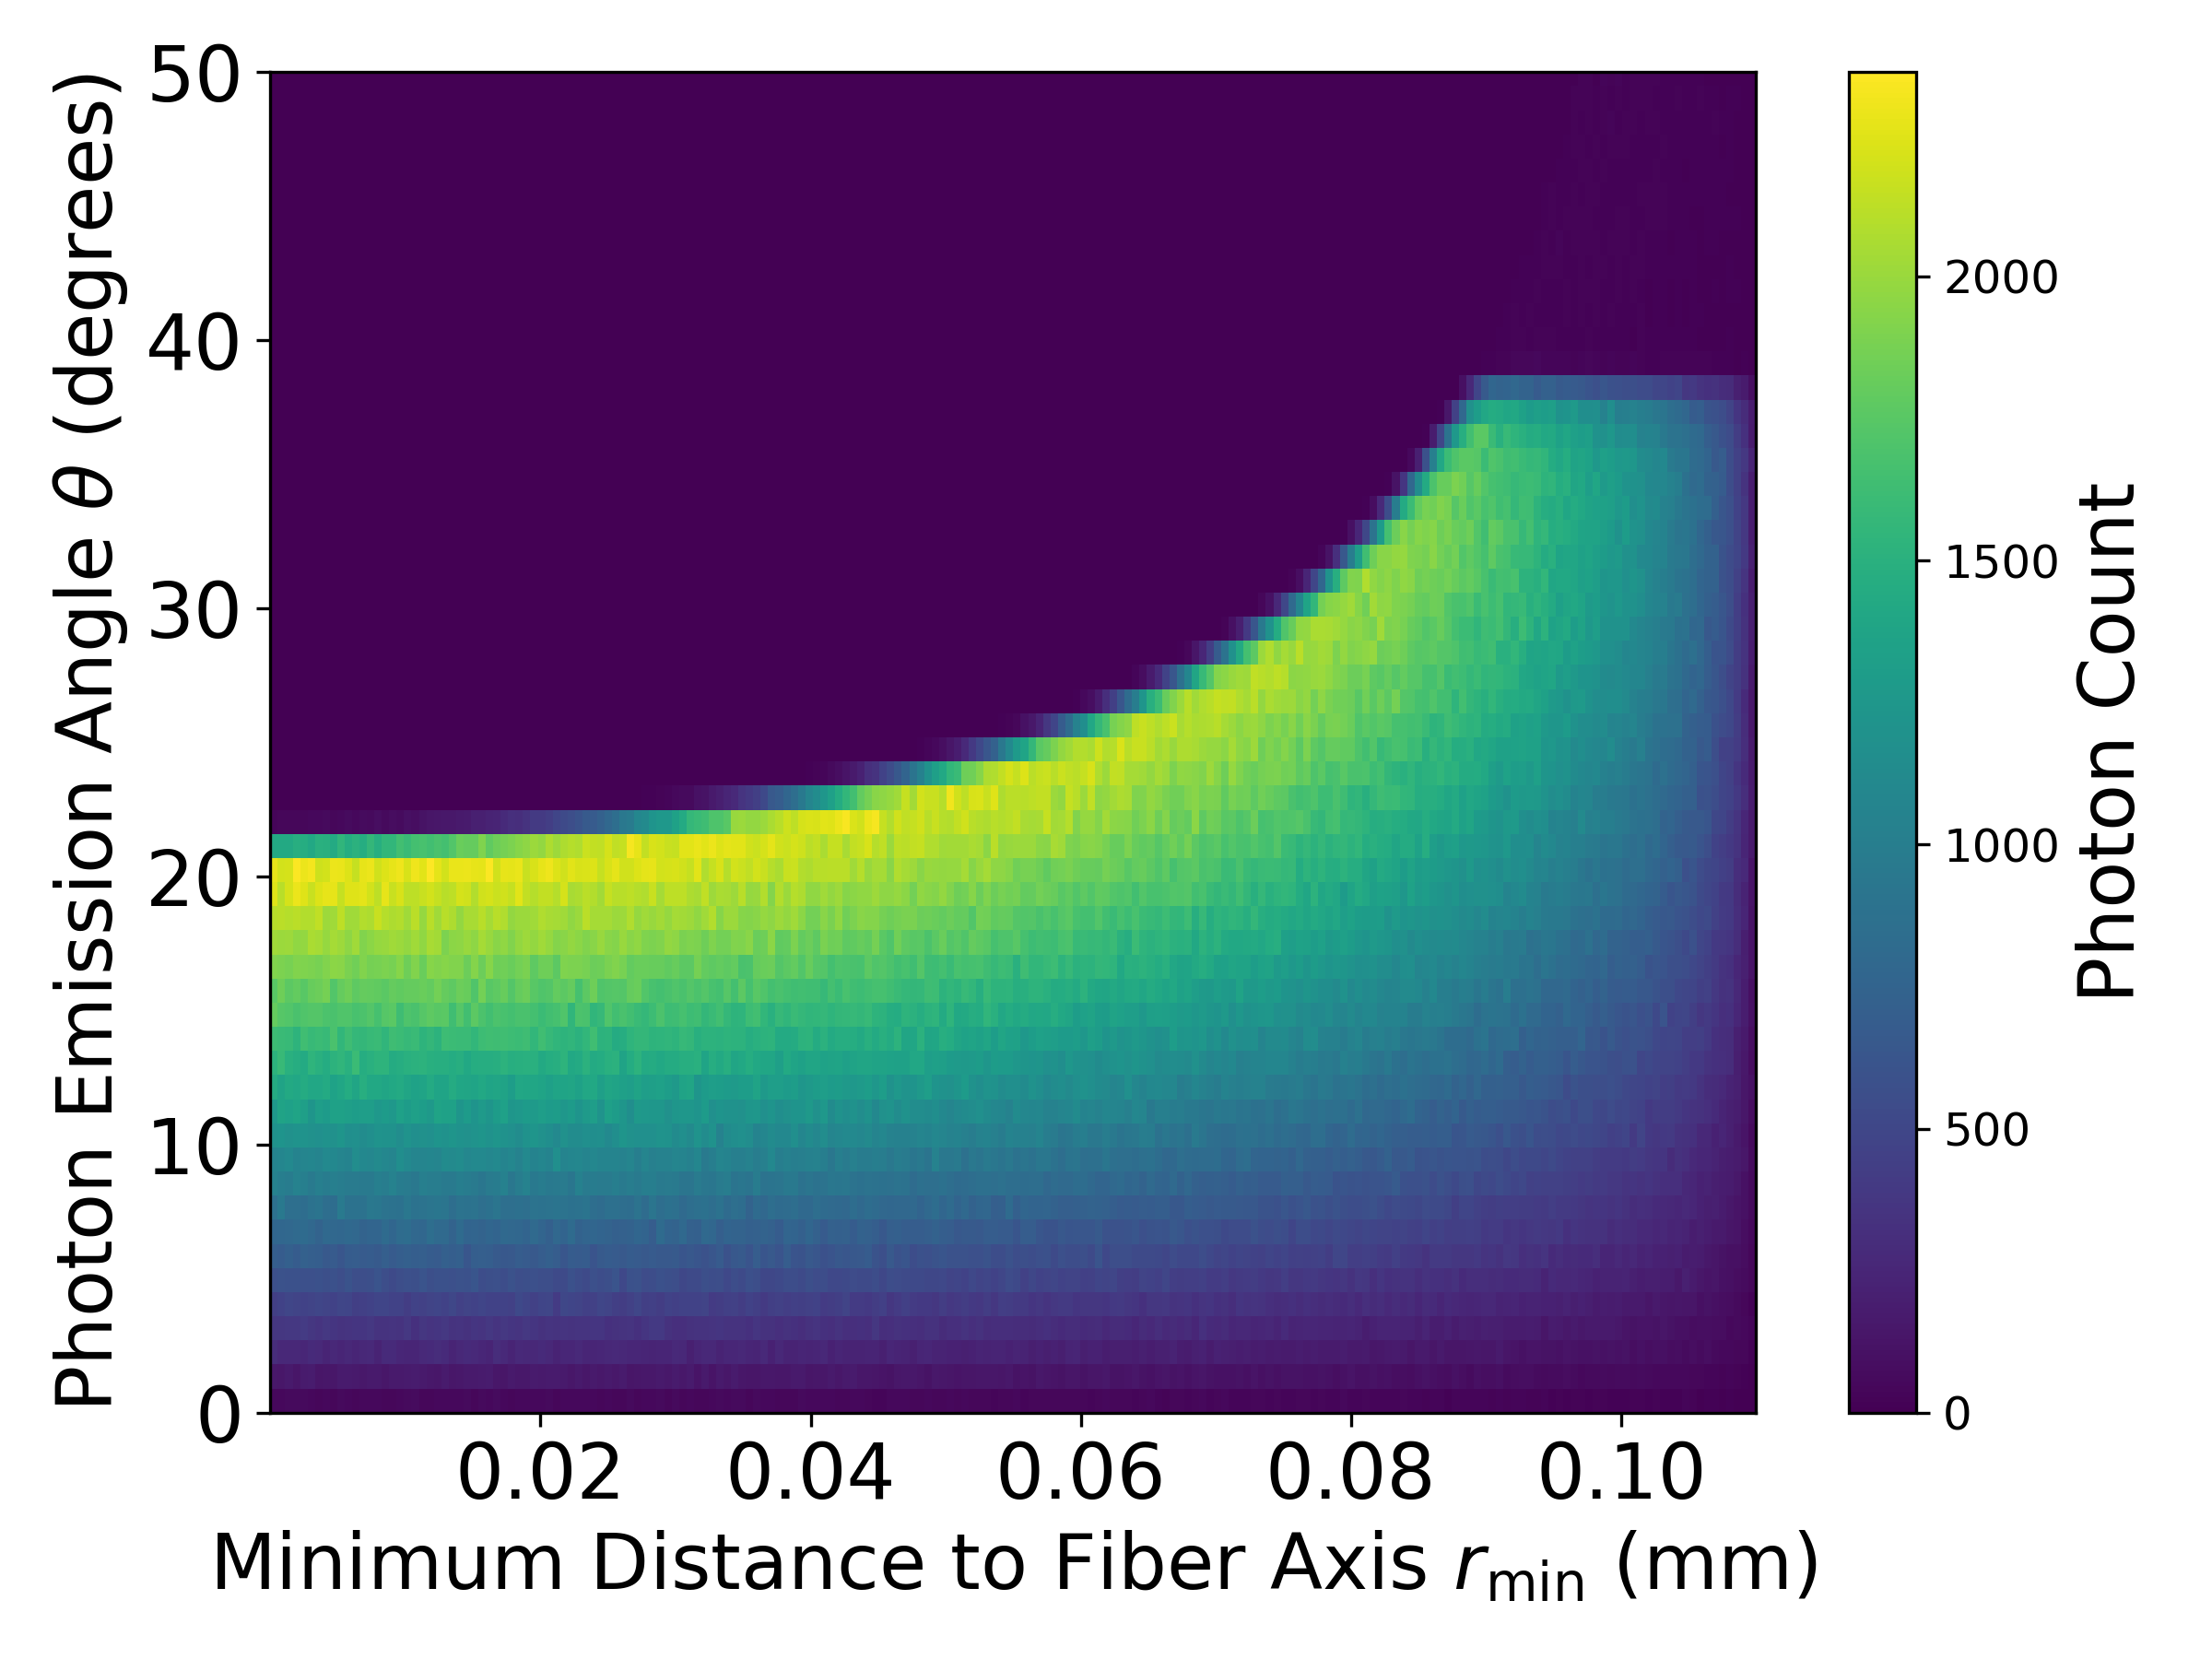
\includegraphics[width=\textwidth, scale=0.35]{Figure/rmin_vs_theta_histogram.png}
        \caption{For core photons}
        \end{subfigure}
        \hfill
        \begin{subfigure}[b]{0.48\textwidth}
            \centering
            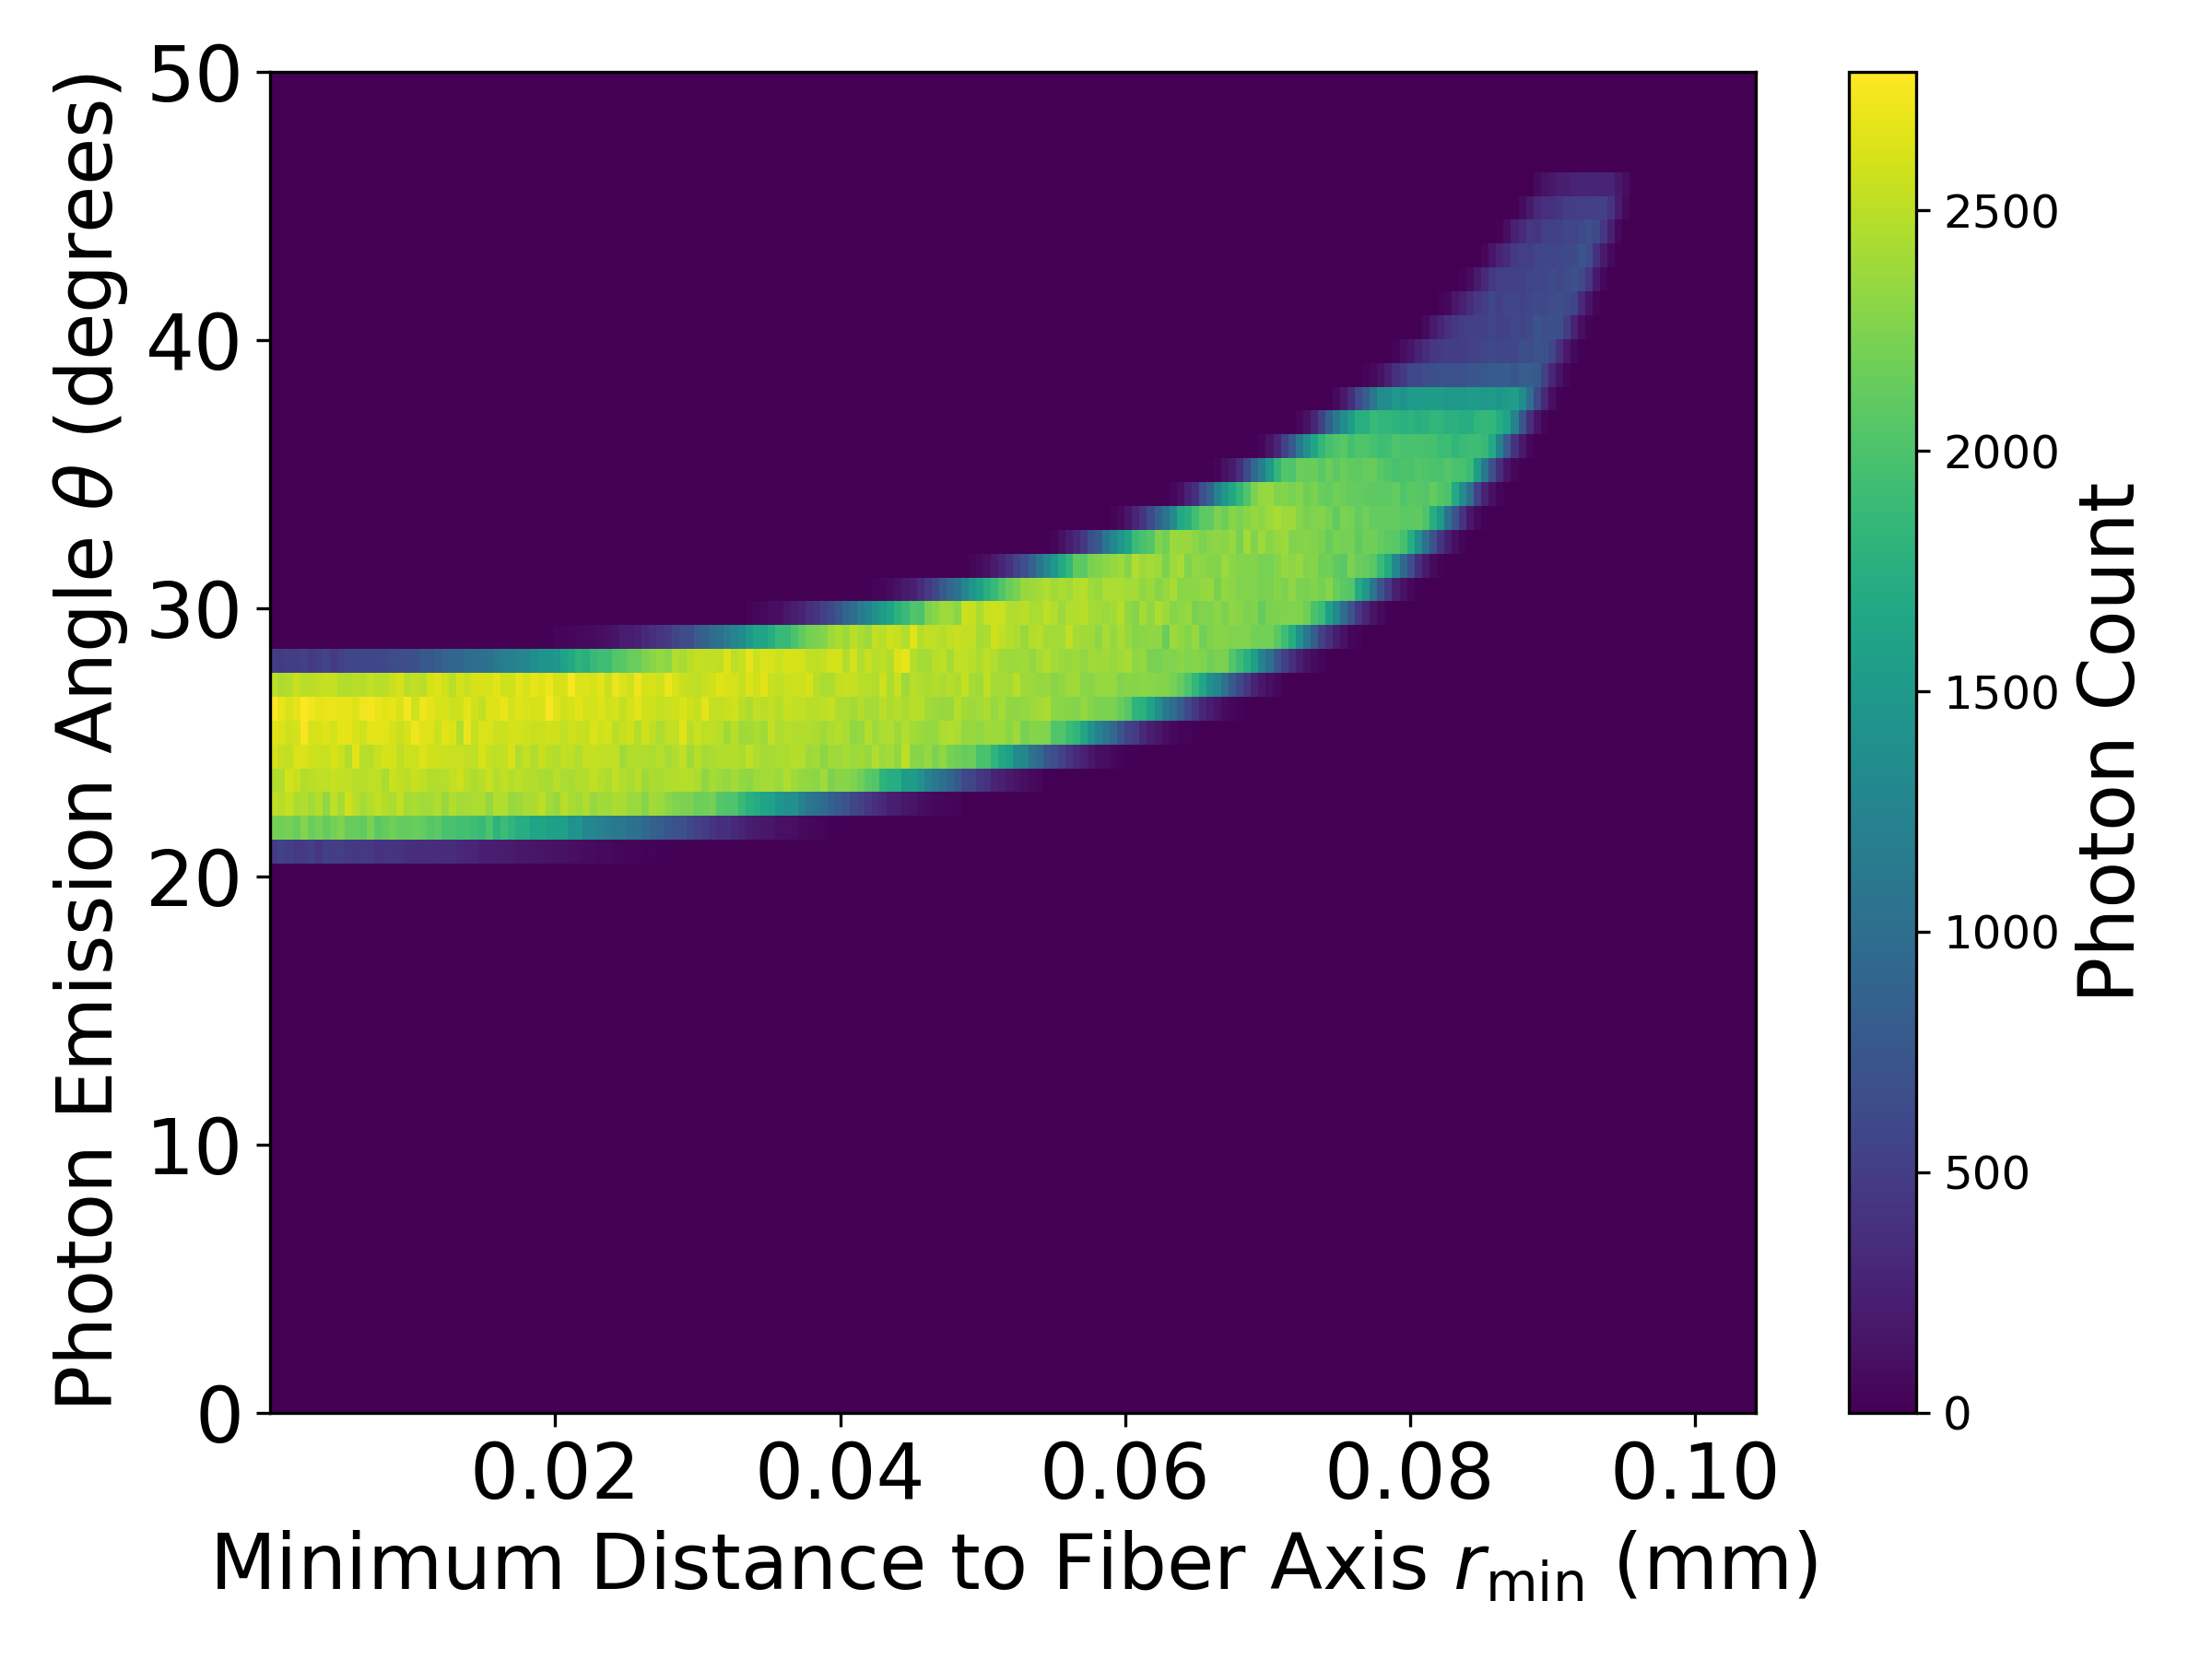
\includegraphics[width=\textwidth, scale=0.35]{Figure/rmin_vs_theta_histogram_cladding.png}
            \caption{For cladding photons}
        \end{subfigure}
        \caption{Heatmaps of photon intensity distribution with respect to distance \( r_{\text{min}} \) and emission angle \( \theta \) from the fiber axis.}
        \label{dist_1}
    \end{figure}

    At any given \( r_{\text{min}} \) for core photons, the intensity varies depending on the emission angle of the photon. The sharp edges are indicative of the critical angle at which total internal reflection reaches the layer boundaries. Nevertheless, for cladding photons, the intensity is confined to a specific region. The pattern arises from the fact that cladding photons are guided within the cladding layer. The confinement characteristic is crucial in protecting photon energy loss from the core and ensuring that the light is guided through the fiber. \\

    %Explain how to fit the data and the results %
    
    Furthermore, the detected photon intensity shows a clear dependence on the excitation position \( X \). As illustrated in Figure \ref{dist_2}, the distributions strongly support this relationship and provide a way to determine the attenuation length.
    
    \begin{figure}[H]
        \centering
        \begin{subfigure}[b]{0.48\textwidth}
            \centering
            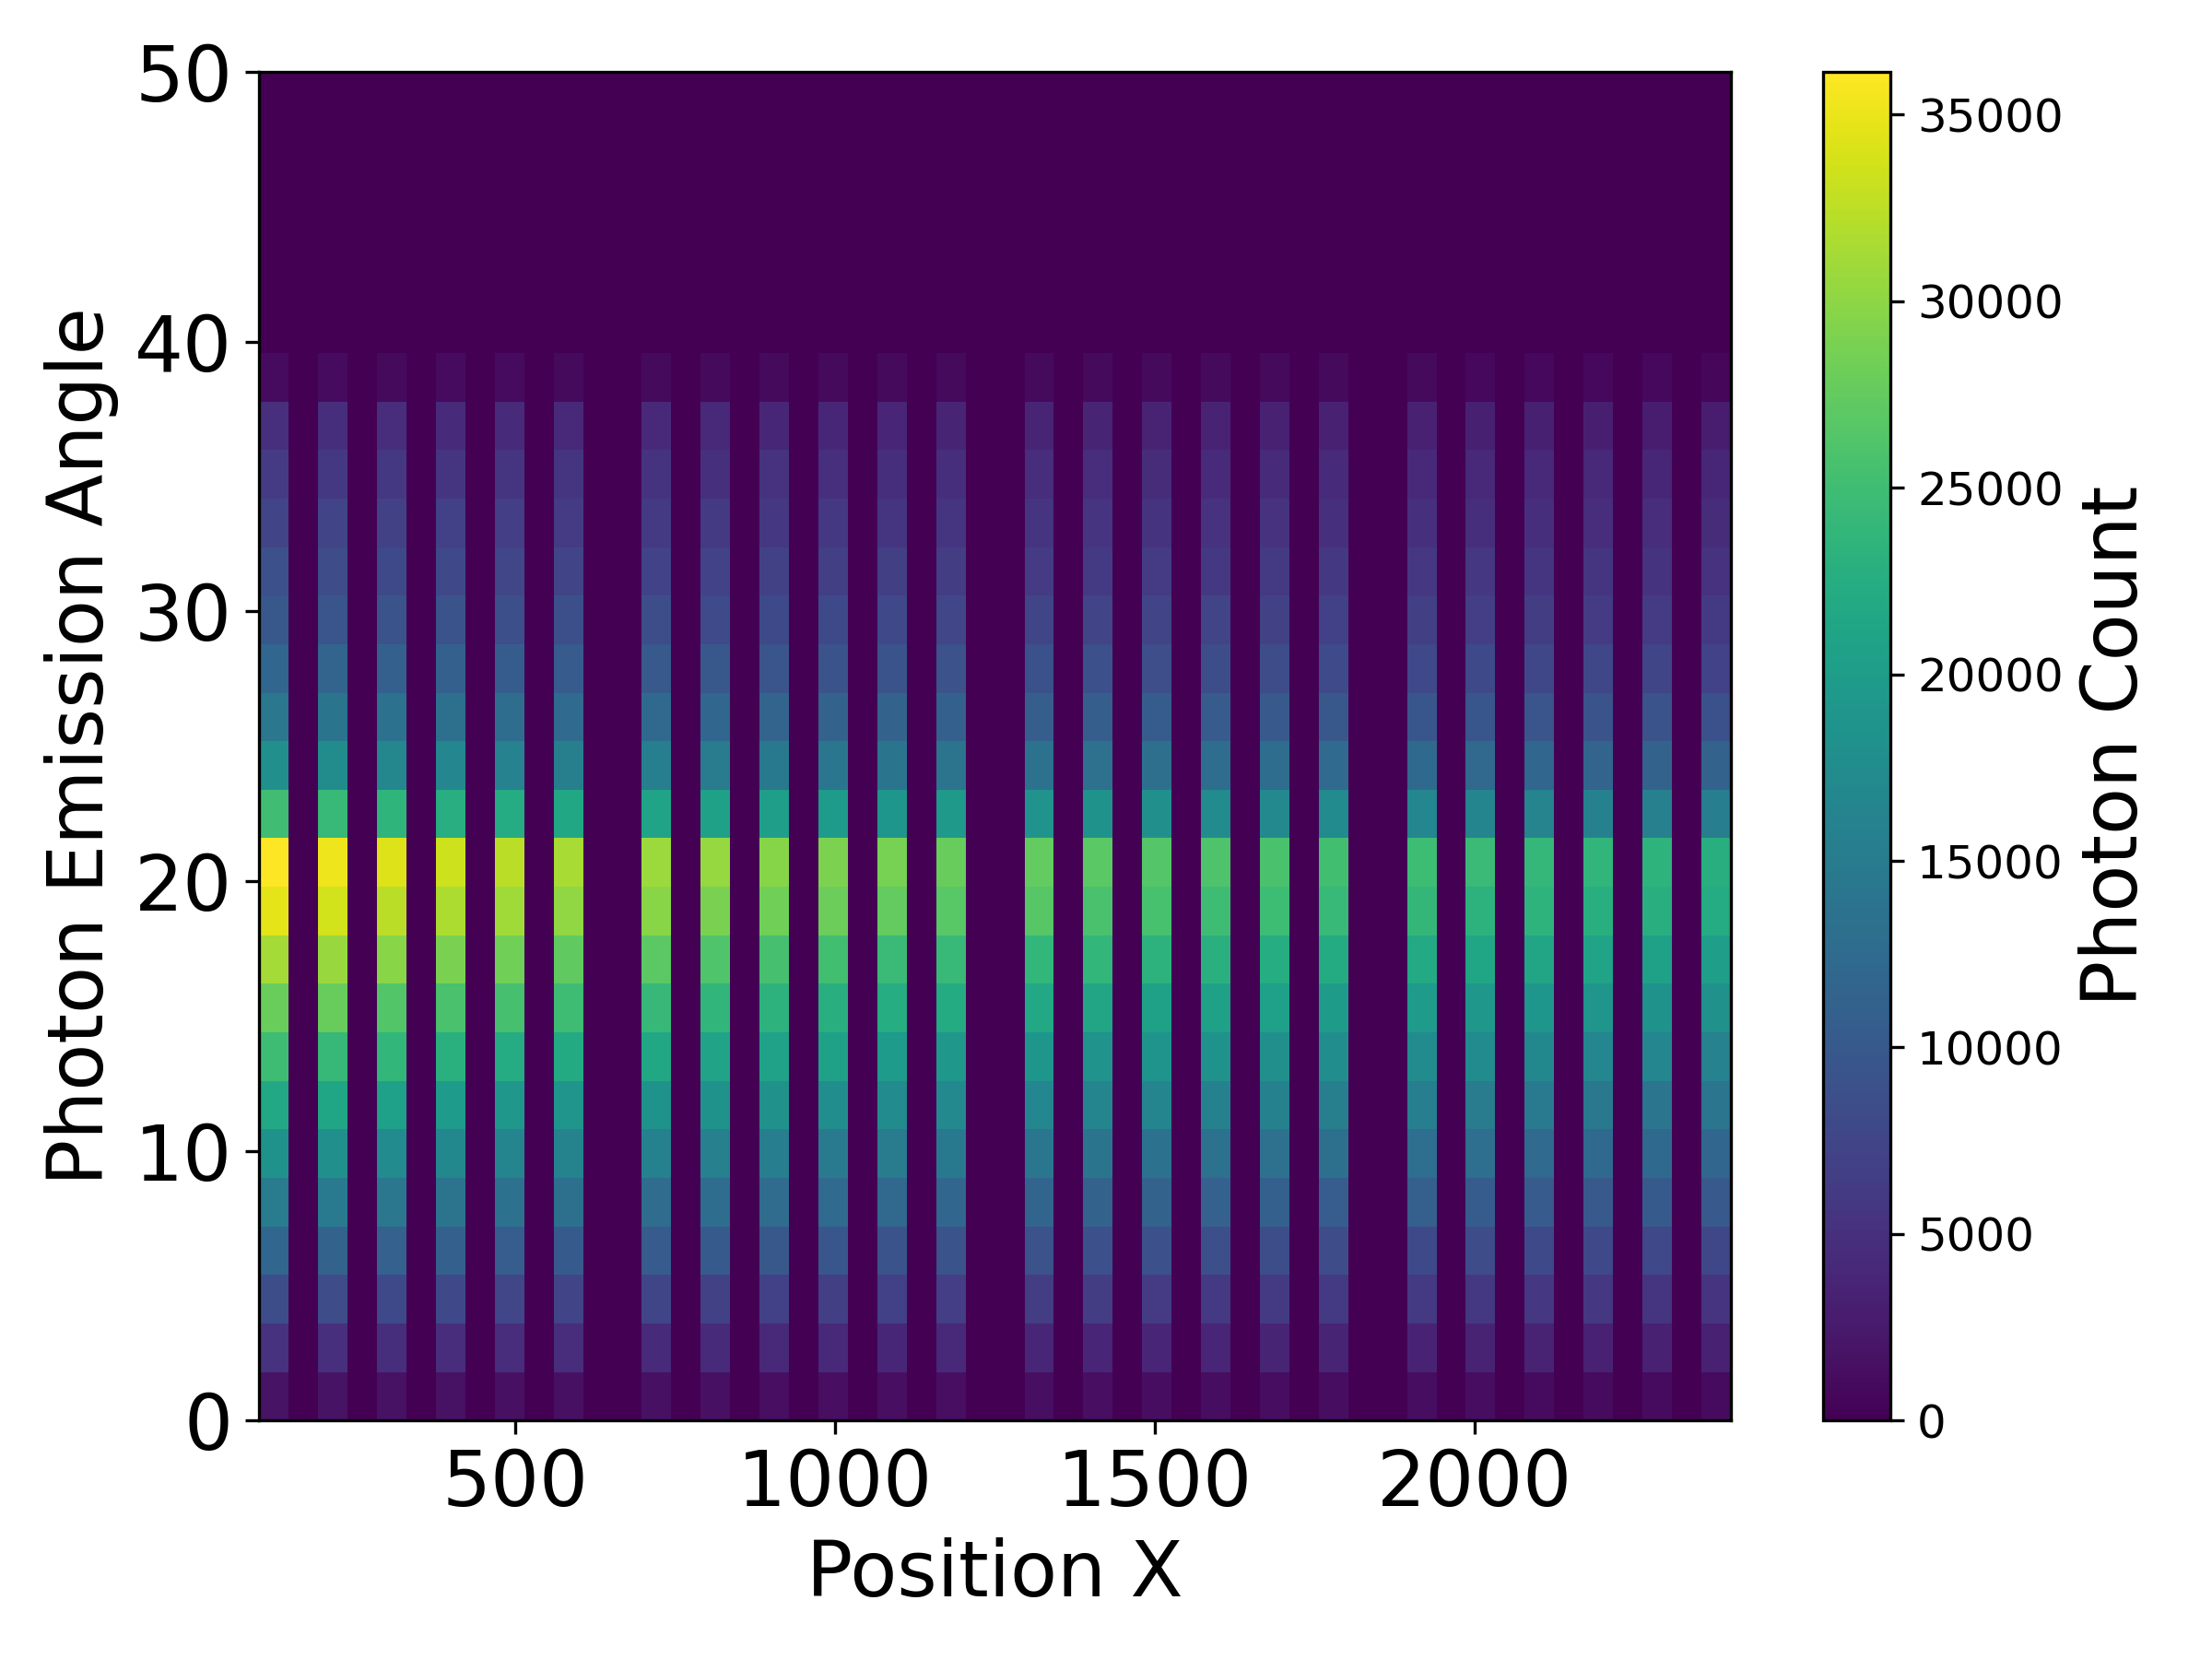
\includegraphics[width=\textwidth, scale=0.35]{Figure/exciting-core.png}
            \caption{For core photons}
        \end{subfigure}
        \hfill
        \begin{subfigure}[b]{0.48\textwidth}
            \centering
            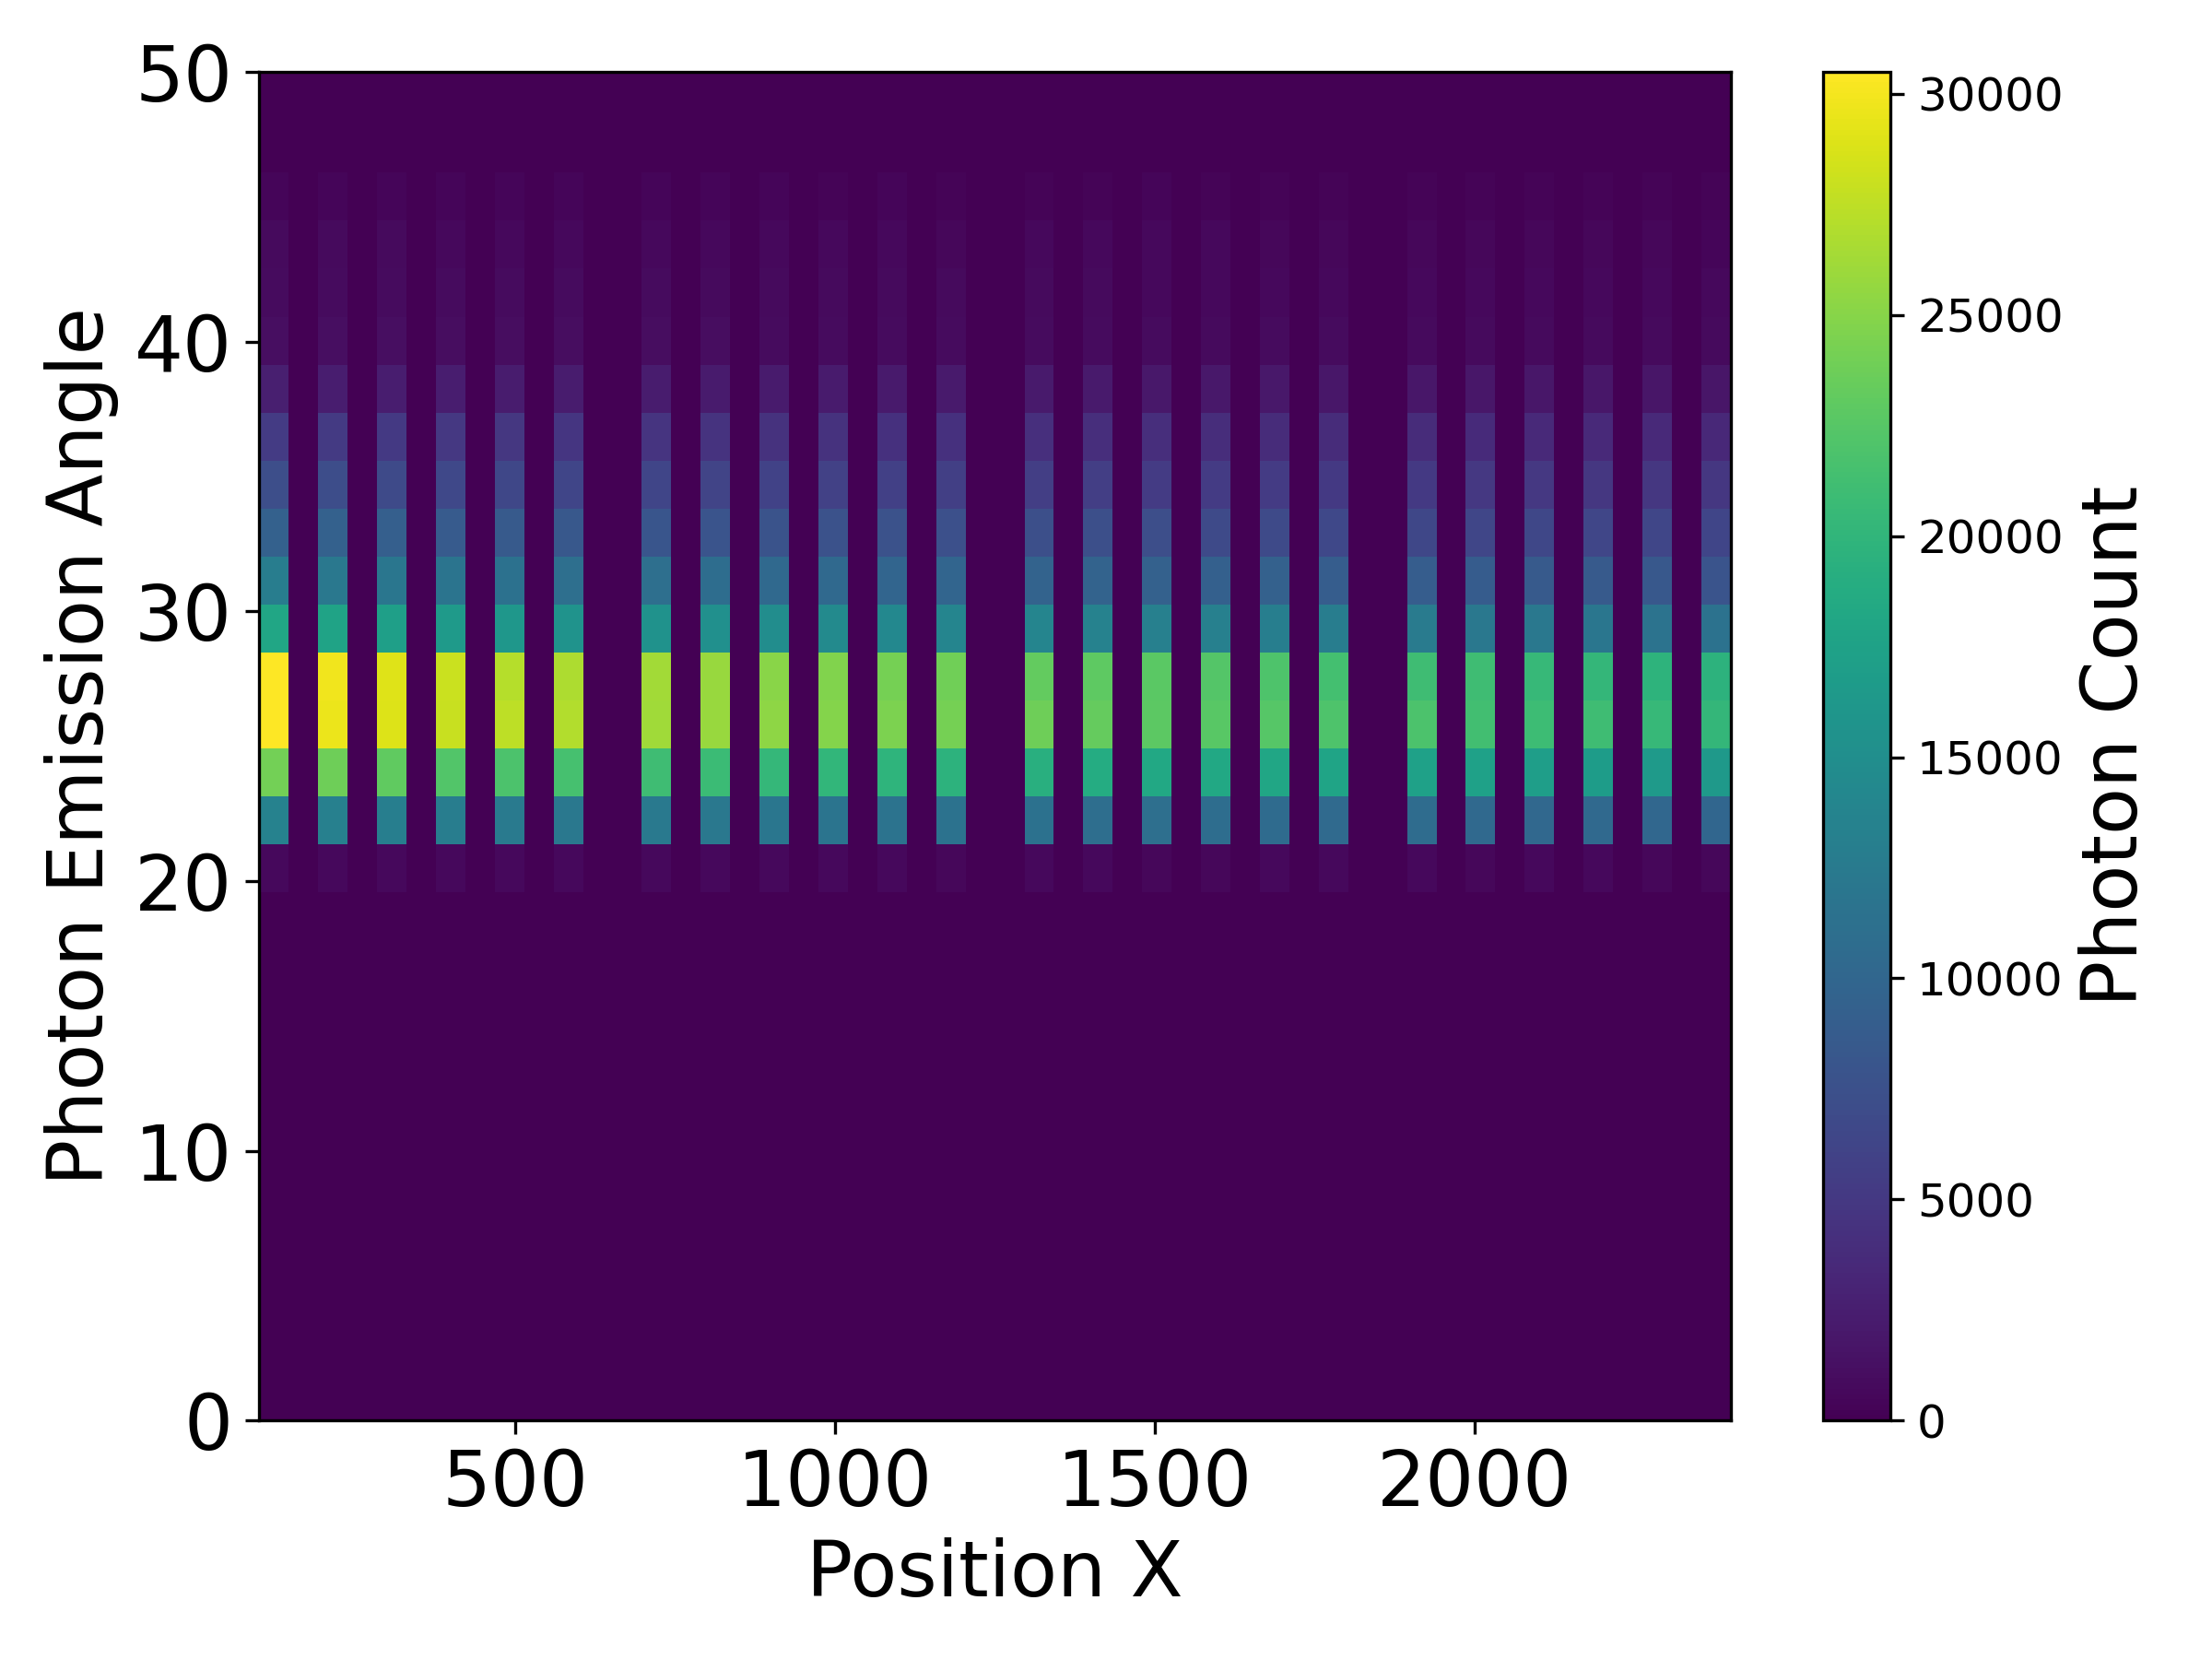
\includegraphics[width=\textwidth, scale=0.35]{Figure/exciting-clad.png}
            \caption{For cladding photons}
        \end{subfigure}
        \caption{Heatmaps of photon intensity distribution with respect to distance \( r_{\text{min}} \) and position $X$ from the fiber axis.}
        \label{dist_2}
    \end{figure}

    The attenuation of photons refers to the reduction in the intensity of photons as they travel through a medium. Practically, the intensity is expected to decrease depending on the excitation position and angle. Figure \ref{dist_2} provides an idea of the relationship, which should be considered as an exponential function. Theoretically, the attenuation of photons after traveling a path length $x$ in the fiber is described by

    \begin{equation}
    I(x) = I_0 e^{-\frac{x}{L}}
    \label{eq:attenuation}
    \end{equation}

    where $L$ is the attenuation length. In the analysis, the simulated data for both core and cladding photons will be grouped based on their excitation angles and fitted using the equation $\ref{eq:attenuation}$. The fitting curves are shown in Figure \ref{fit_1}. For core photons, the attenuation length ranges from 4800 mm to 5150 mm, while for cladding photons it ranges from 5200 mm to 6400 mm. The result is understandable because the cladding often has a lower energy absorption coefficient than the doped core.


\begin{figure}[H]
    \centering
    \begin{subfigure}[t]{0.9\textwidth}
        \centering
        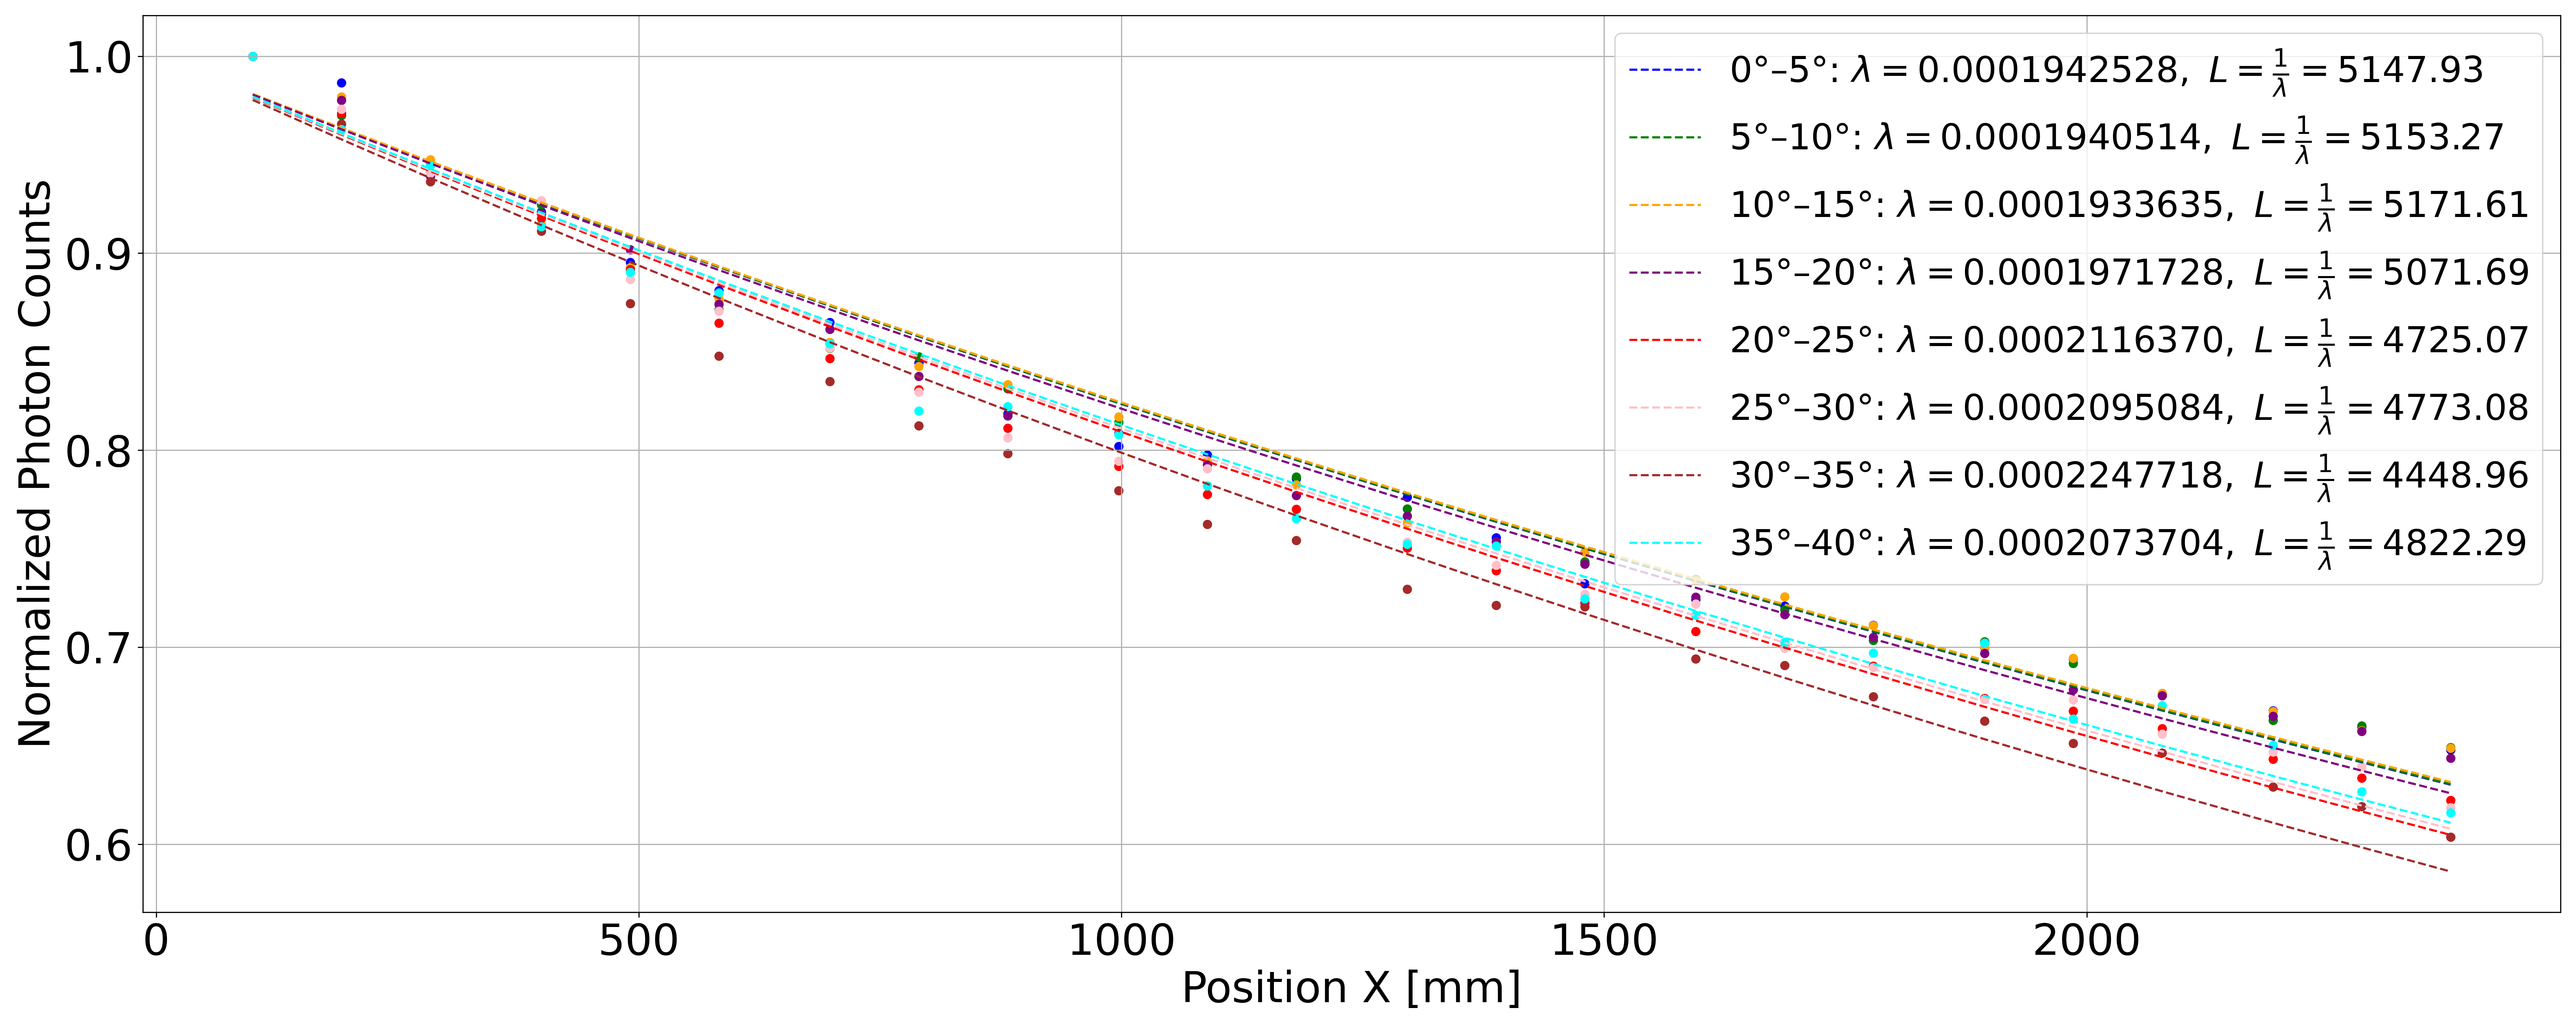
\includegraphics[width=\textwidth]{Figure/fit_40_core.png}
        \caption{For core photons}
    \end{subfigure}
    
    \vspace{1em}  % Add vertical space between the two subfigures

    \begin{subfigure}[t]{0.9\textwidth}
        \centering
        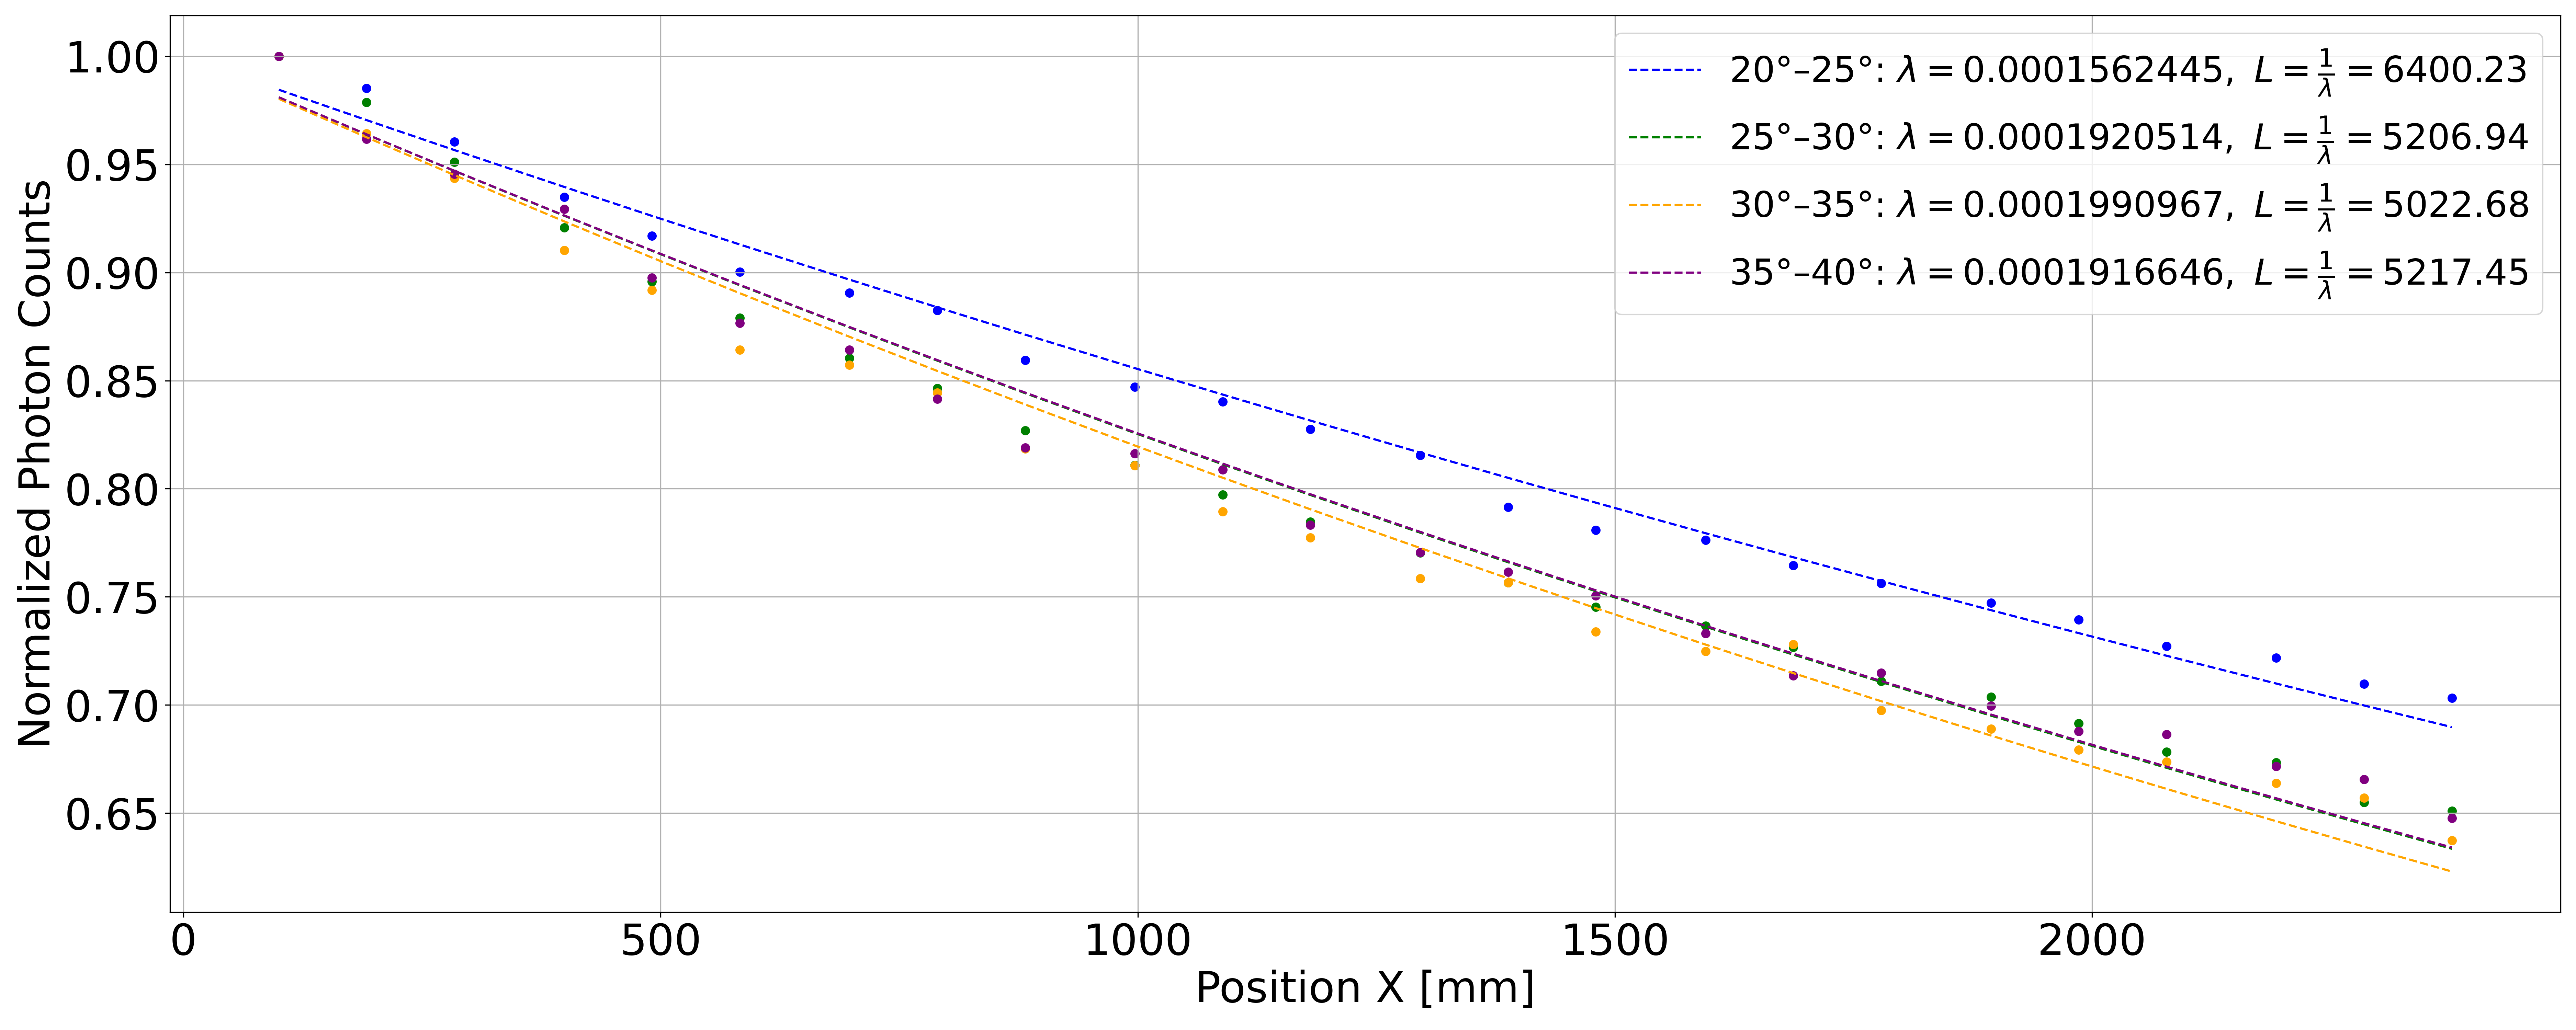
\includegraphics[width=\textwidth]{Figure/fit_40_clad.png}
        \caption{For cladding photons}
    \end{subfigure}

    \caption{
        Graph of the normalized photon intensity versus position \( x \), showing exponential fits to simulation data for core and cladding photons.
    }
    \label{fit_1}
\end{figure}

    In conclusion, the simulation data serve as a quantitative benchmark for the guidance and analysis of experimental data in the next measurement.
    
    \section{Intensity Measurement}
    The purpose of the last experiment is to measure the light intensity at various horizontal angles and excitation positions to determine the attenuation length of the scintillating fiber. The horizontal intensity was measured over angles from \( 0^\circ \) to \( 36^\circ \), and the excitation positions were varied from \( 10\,\text{mm} \) to \( 1960\,\text{mm} \). \\

    Unfortunately, as shown in Figure \ref{jump}(left), the experimental data exhibited a discontinuous curve, whereas it is theoretically expected to be continuous. The observed discontinuity may be attributed to damages of the fibers. To reconstruct the data, for each point in the dataset, the median of the differences between all pairs of points will be added to the point. Such median is calculated by first computing the absolute differences \( \Delta x = |x_i - x_j| \) for all pairs of points \( (x_i, x_j) \). Then, the differences that satisfy the condition \( \Delta x \geq 2 \times \sigma \) would be selected to calculate the median, where \( \sigma \) is the standard deviation of the dataset. Figure~3--7 (right) presents the corrected graph of photon intensity versus excitation position \( x \).


    \begin{figure}[H]
        \centering
        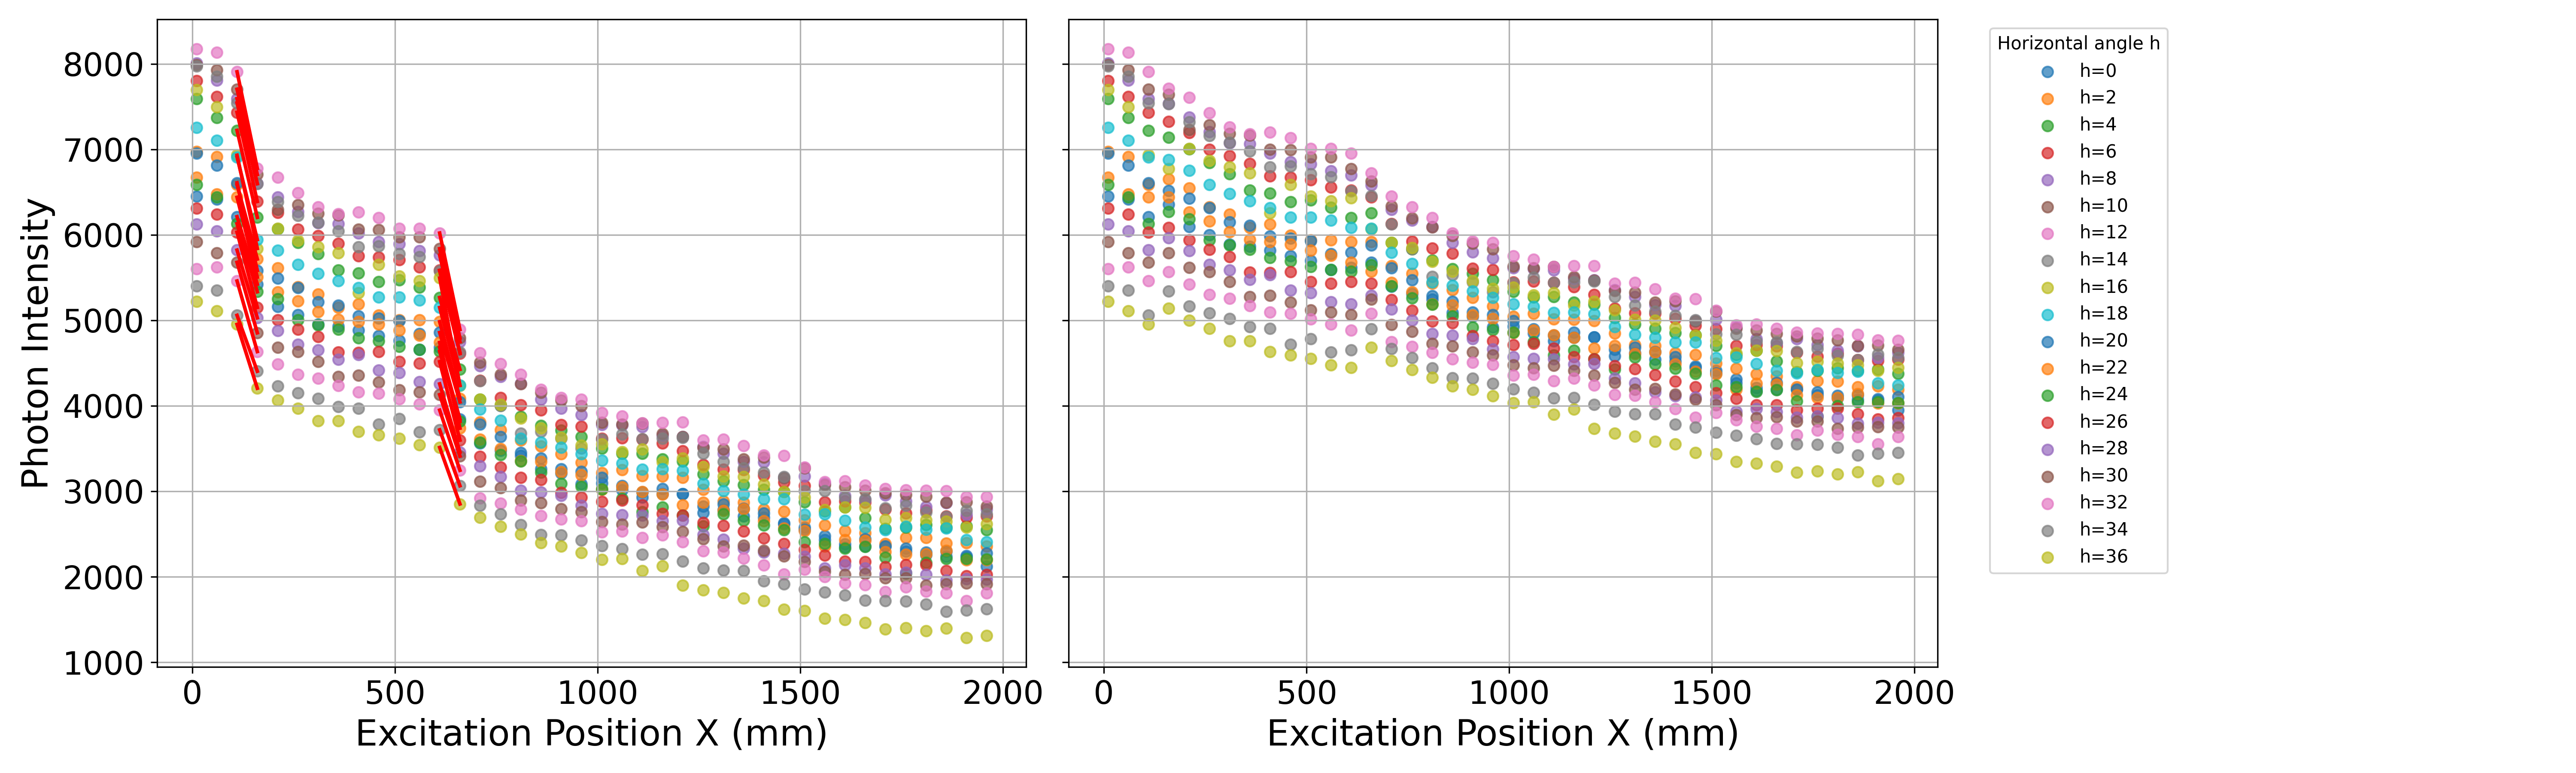
\includegraphics[scale=0.4]{Figure/jump.png}
        \caption{Graph of the  photon intensity versus position \( x \)}.
        \label{jump}
    \end{figure}

    The length of the attenuation will be determined using the reconstructed experimental data. Equation \(\ref{eq:attenuation}\) is applied in an exponential fit that would be performed for each horizontal angle. Figure \ref{l} shows a scatter plot of the attenuation length versus the horizontal angle. The pattern observed in the figure is consistent with the simulation results, where the attenuation length is dependent on the excitation angles, thus influencing the horizontal angle.
    
    \begin{figure}[H]
        \centering
        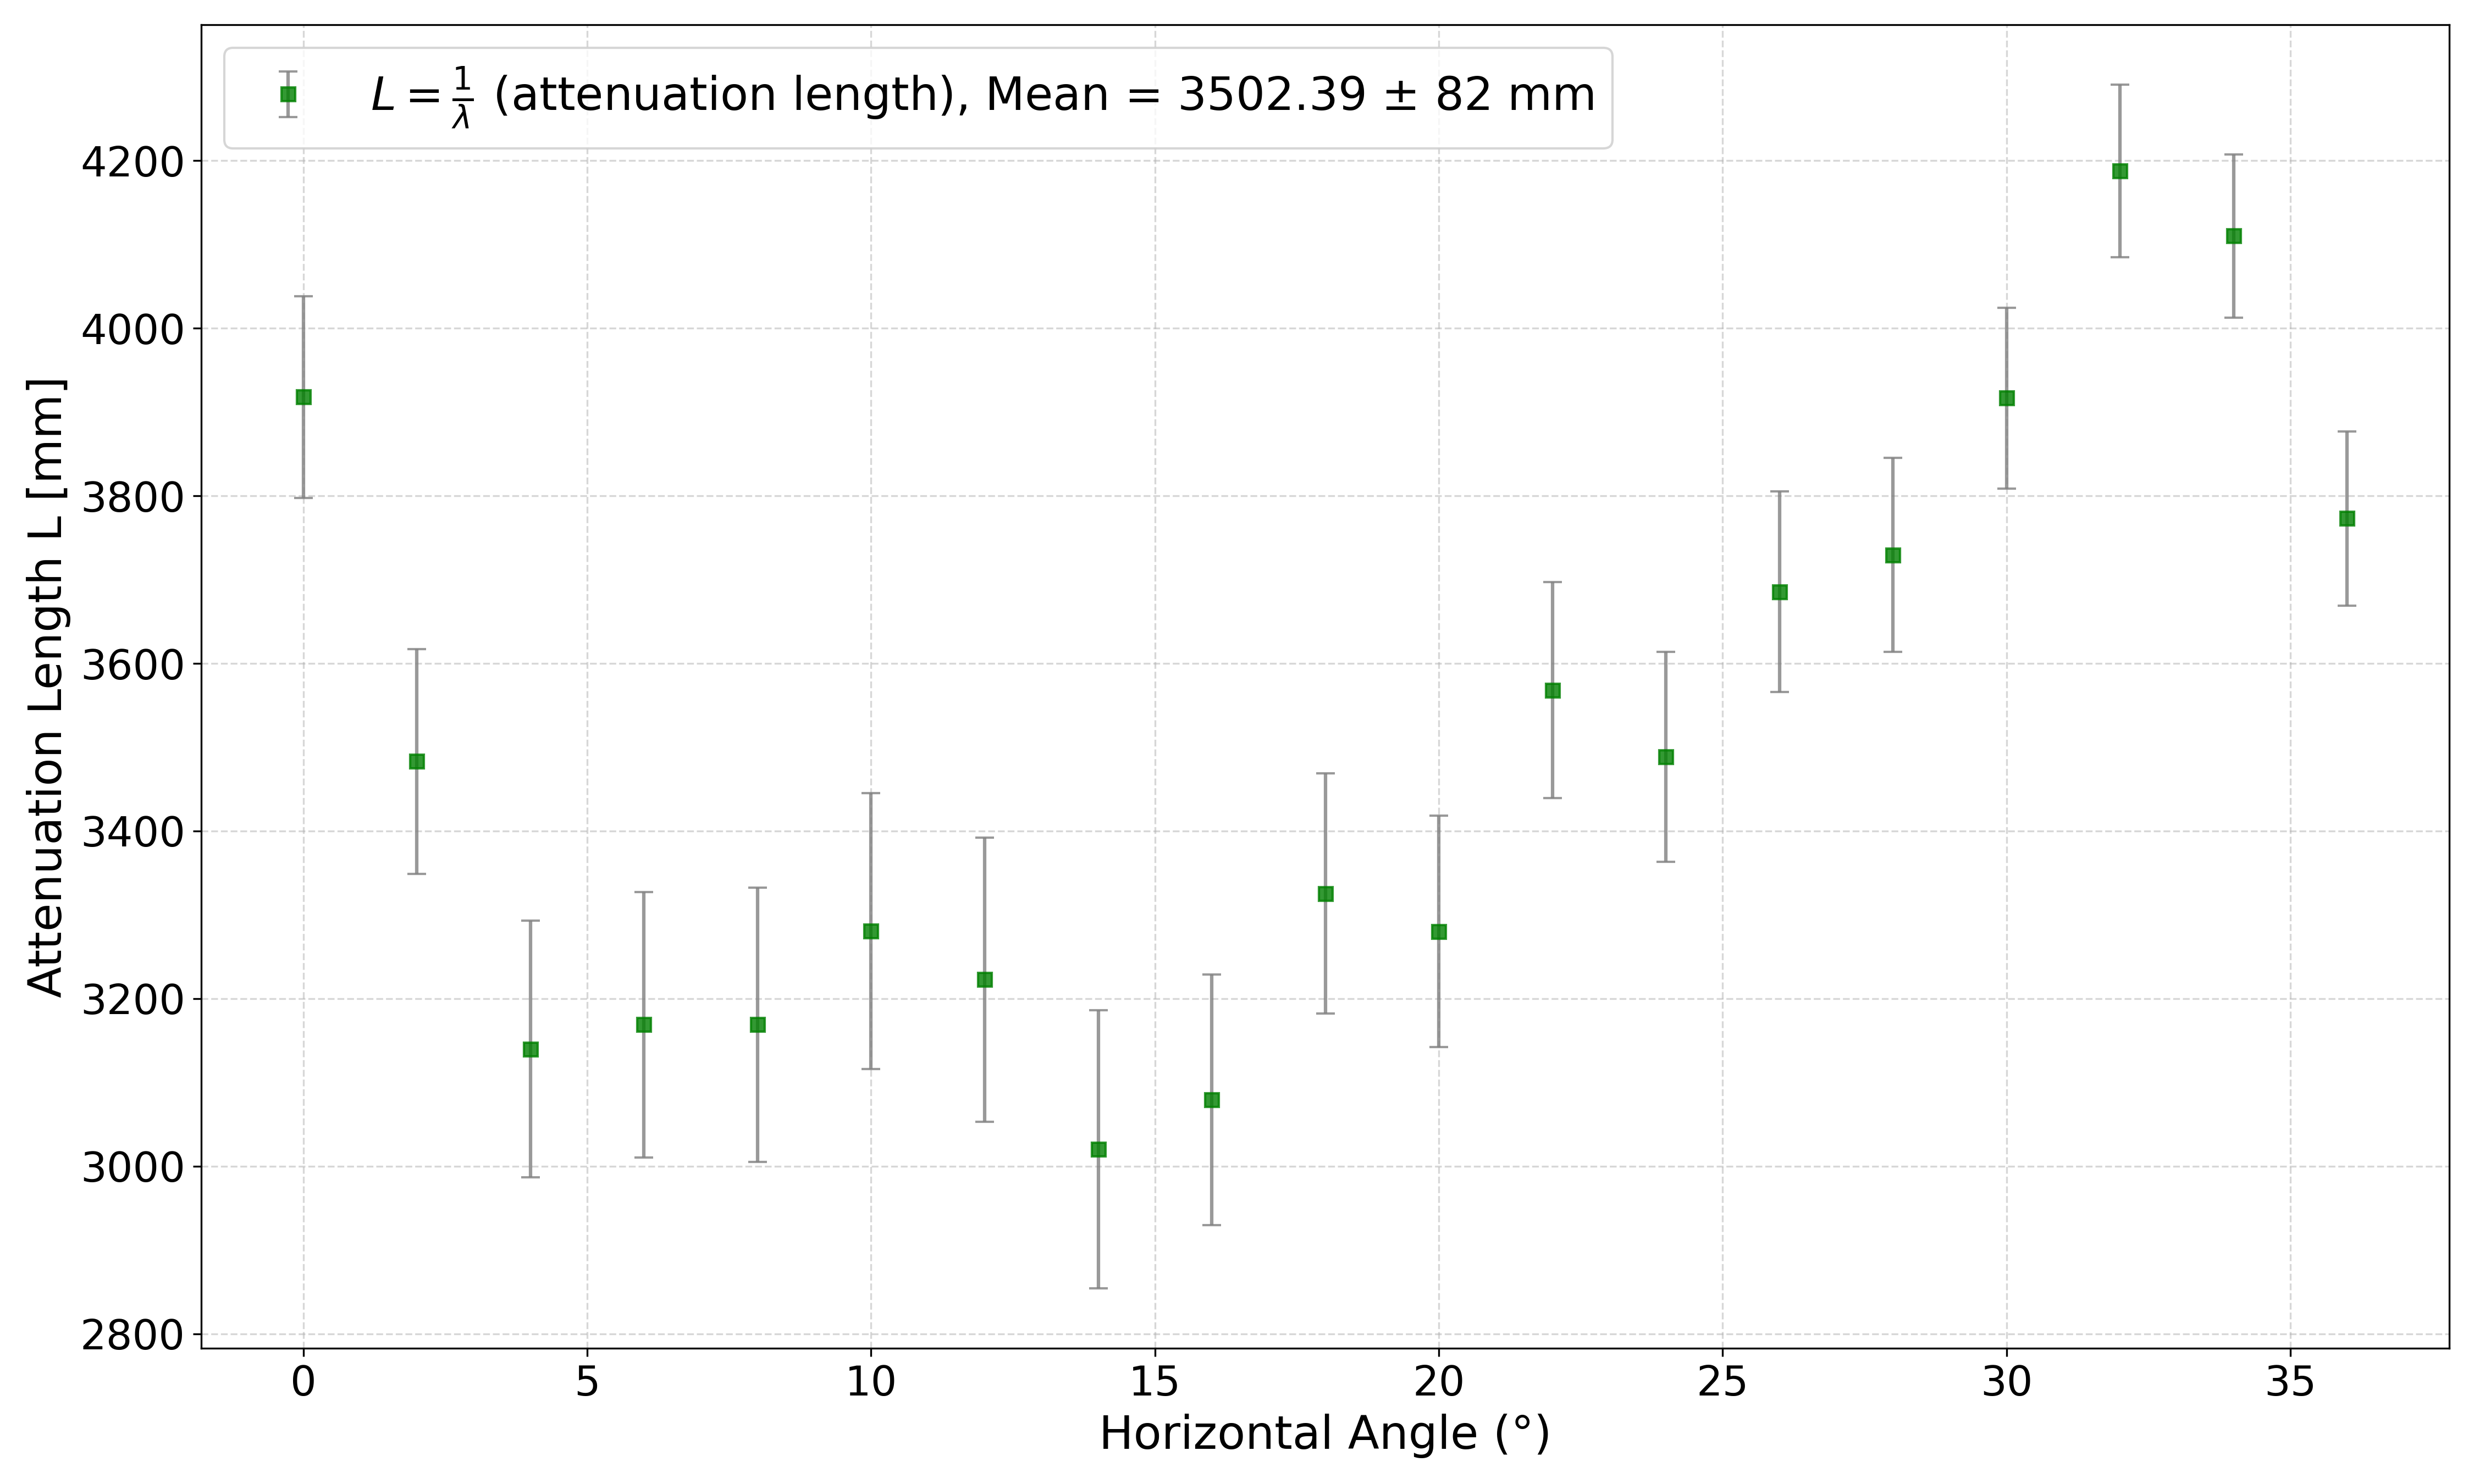
\includegraphics[scale=0.3]{Figure/l-fit.png}
        \caption{Scatter plot of the attenuation length versus the horizontal angle}
        \label{l}
    \end{figure}

    The attenuation length ranges from 3,000 $mm$ to 4,200 $mm$, which is quite consistent with the simulation data in the previous analysis. The average attenuation length is $3,502.39 \pm 82\ \mathrm{mm}$, as expected from this type of scintillating fibre.
    
    % 
    % In the end, the measured attenuation length will be compared with simulation results to assess the fiber's performance and accuracy.
